\documentclass[12pt]{article}
\usepackage[utf8]{inputenc}
\usepackage[left=2.5cm, right=2.5cm, top=2.0cm]{geometry}
\usepackage{sectsty}
\usepackage{graphicx}
\usepackage{amsmath}
\usepackage{amssymb}
\usepackage{undertilde}
\usepackage{kbordermatrix}
\usepackage{listings}
\usepackage{ulem}
\usepackage{soul}
% \usepackage{tikz}
% \usepackage{pgfplots}
% \pgfplotsset{compat=1.16}
\usepackage{siunitx}
\usepackage{pythonhighlight}
\usepackage{caption}
\usepackage{float}
\usepackage{url}
\usepackage{enumitem}
\usepackage{bm}
\usepackage{empheq}
\usepackage{tcolorbox}
\usepackage{framed}
\usepackage{xparse}
\usepackage{algorithm, algorithmic}
% \usepackage{algorithmic}
\usepackage{booktabs}
\usepackage{tabularx}
% ref packages
\usepackage{nameref}
% folowing  must be in this order
\usepackage{varioref}
\usepackage{hyperref}
\usepackage{cleveref}
\usepackage{mathtools}
\usepackage{longtable}
\DeclareMathOperator*{\argmax}{arg\,max}
% \usepackage[shortlabels]{enumitem}
\tcbuselibrary{breakable}
\allowdisplaybreaks


%  ---------------------- COMMANDS ---------------------------
% Double underline
\def\dunderline#1{\underline{\underline{#1}}}

% Shorten nonumber command
\def\nnb{\nonumber}

% Shorten boldsymbol command
\def\bs#1{\boldsymbol{#1}}

% Algorithmic newline
\def\algonewline{\STATE{ }}

% Eigenvectors of
\def\eigvecof{\text{eigenvectors of }}

% Eigenvalues of 
\def\eigvalof{\text{eigenvalues of }}

% Enclose in square brackets
\newcommand{\enclb}[1]{\left[#1\right]}
% Enclose in parenthesis
\newcommand{\enclp}[1]{\left(#1\right)}
% Enclose in curly brackets
\newcommand{\enclc}[1]{\left\{#1\right\}}

% Annotate first argument, text in second argument
\newcommand{\overtext}[2]{\overbrace{#1}^{\mathclap{\text{#2}}}}
\newcommand{\undertext}[2]{\underbrace{#1}_{\mathclap{\text{#2}}}}

% Normalization constant in multivariate normal
\newcommand{\mvnconst}[1]{\frac{1}{(2\pi)^{d/2} |#1|^{1/2}}}

% Exponential factor in multivariate normal
\newcommand{\mvnexpo}[3][x]{\exp \left[  -{\frac{1}{2}} (#1 - #2)^T #3^{-1} (#1 - #2) \right]}

% Multivariate normal
\newcommand{\mvn}[3][x]{\mvnconst{#3} \mvnexpo[#1]{#2}{#3}}

% For numbering in align* environment
\newcommand{\numberthis}{\addtocounter{equation}{1}\tag{\theequation}}

%  Sum notation w/ limits as argument and index as option
\newcommand{\sumlim}[3][i]{\sum\limits_{#1=#2}^{#3}}

%  Product notation w/ limits as argument and index as option
\newcommand{\prodlim}[3][i]{\prod\limits_{#1=#2}^{#3}}

%  Sum notation with only information beneath
\newcommand{\sumnolim}[1]{\sum\limits_{#1}}

%  Integral notation w/ limits as argument and index as option
\newcommand{\intlim}[2]{\int\limits_{#1}^{#2}}

%  Integral over whole domain notation, no args
\newcommand{\intinf}{\int\limits_{-\infty}^{\infty}}

%  Partial derivative notation, arg1: numerator, arg2: denominator
\newcommand{\pfrac}[3][ ]{\frac{\partial^{#1} #2}{\partial #3^{#1}}}

%  Derivative notation, arg1: numerator, arg2: denominator
\newcommand{\dvfrac}[3][ ]{\frac{\text{d}^{#1} #2}{\text{d} #3^{#1}}}

% When doing Gauss-Jordan, create arrow showing operations
\newcommand{\ro}[1]{\xrightarrow{\mathmakebox[\rowidth]{#1}}}

% ----------------------INVIRONMENTS---------------------------
% Item list with title
\newenvironment{titlemize}[1]{%
  \paragraph{#1}
  \begin{itemize}}
  {\end{itemize}}

  % Enum list with title
\newenvironment{titleenum}[1]{%
  \paragraph{#1}
  \begin{enumerate}}
  {\end{enumerate}}

  % Augmented matrix (matrix with vertical line)
\newenvironment{sysmatrix}[1]
  {\left(\begin{array}{@{}#1@{}}}
  {\end{array}\right)}

 % Make matrices with more spacing
\makeatletter
\renewcommand*\env@matrix[1][\arraystretch]{%
  \edef\arraystretch{#1}%
  \hskip -\arraycolsep
  \let\@ifnextchar\new@ifnextchar
  \array{*\c@MaxMatrixCols c}}
\makeatother

% \renewcommand*{\arraystretch}{1.5}

\newlength{\rowidth}% row operation width
\AtBeginDocument{\setlength{\rowidth}{3em}}

\floatname{algorithm}{Algorithm}
\renewcommand{\algorithmicrequire}{\textbf{Input:}}
\renewcommand{\algorithmicensure}{\textbf{Output:}}

\begin{document}
\title{\textbf{INF367A Project 1}}
\author{Naphat Amundsen}
\maketitle
\sectionfont{\fontsize{14}{15}\selectfont}
\subsectionfont{\fontsize{12}{15}\selectfont}
\subsubsectionfont{\fontsize{12}{15}\selectfont}
\graphicspath{ {./images/} }

\ifx
\begin{figure}[H]
	\centering
	\includegraphics[scale=0.8]{Figure_2}
	\caption{Insert caption here}
\end{figure}
\fi
\ifx
\begin{figure}[H]
	\centering
	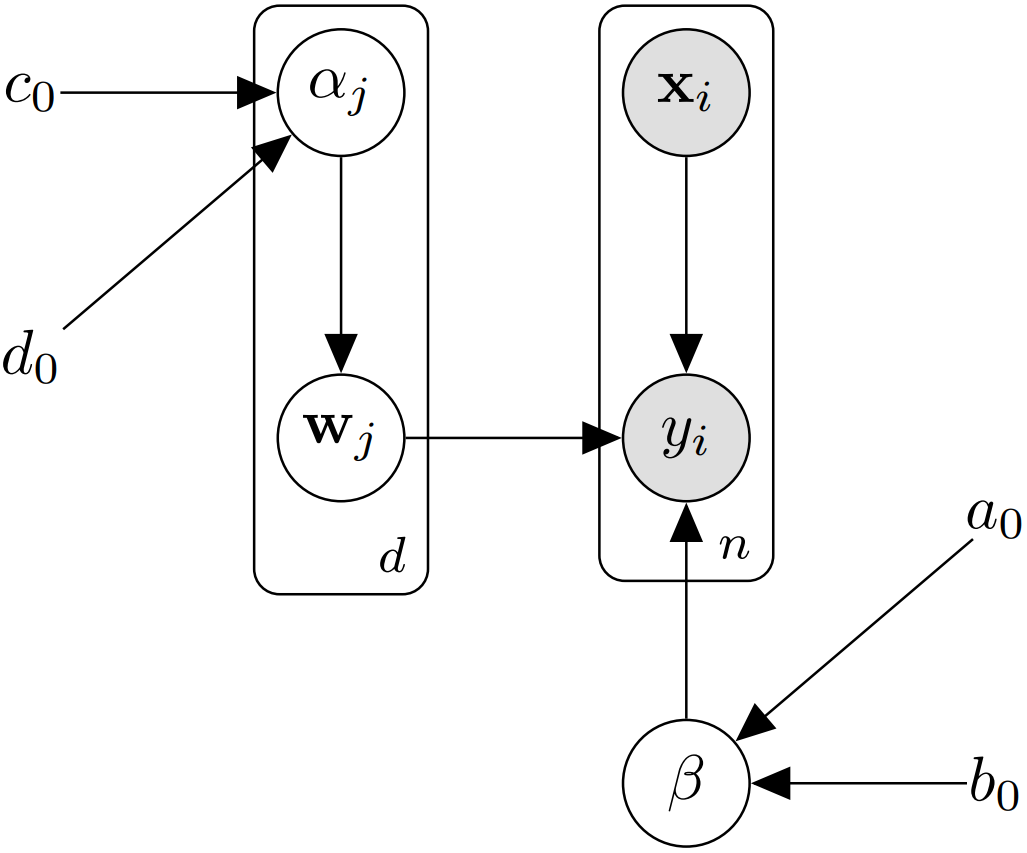
\includegraphics[scale=0.8]{bn_network.png}
	\caption{Plate diagram of the regression model with ARD prior. Variables $x_i$ , and $y_i$ are observed; We are interested in the posterior distribution of parameters $w$, $\alpha$ and $\beta$. The constants $a_0$ , $b_0$, $c_0$ , and $d_0$ are user-defined hyperparameters}
\end{figure}
\fi

\newcommand{\opGamma}{\operatorname{Gamma}}

\section*{Introduction}
    This project is about linear regression using automatic relevance determination (ARD) when doing linear regression. The idea of ARD is to use a flexible prior to push weights of the irrelevant features to zero while not penalizing relevant features, as opposed to L2 regularization and similar methods which suppresses the weights to all features equally. ARD can be viewed as weighted regularization with respect to the features. The ARD weights are then parameters that needs to be optimized as well.

    \vspace{5mm}
    Assume that we have observed $n$ pairs $(x_i, y_i)$ where $x_i$ are the feature values and $y_i$ is the label. Let $w \in \mathbb{R}^d$ be the regression weights. The likelihood is
    \begin{align}
        P(y|x,w,\beta) = \prodlim{1}{n} N(y_i|w^Tx_i,\beta^{-1}) \label{eq:likelihood}
    \end{align}
    The noise precision $\beta$, is modelled with a Gamma prior:
    \begin{align}
        P(\beta) = \opGamma(\beta|a_0,b_0) \label{eq:betaprior}
    \end{align}
    where $a_0$ and $b_0$ are user defined hyperparameters.

    The prior for the weights $w$ is a Gaussian distribution
    \begin{align}
        P(w|\alpha_1, \ldots, \alpha_d) = \prodlim[j]{1}{d} N(w_j|0,\alpha_j^{-1}) \label{eq:wprior}
    \end{align}
    Comparing this to the standard way, the precision of the weights is not just a prior scalar, but an actual distribution. The prior for $\alpha_j$ is a Gamma distribution.
    \begin{align}
        P(\alpha_j) = \opGamma(\alpha_j|c_0,d_0) \quad \forall j = 1, \ldots, d \label{eq:alphaprior}
    \end{align}
    where $c_0$ and $d_0$ are user defined hyperparameters.

    \begin{figure}[H]
        \centering
        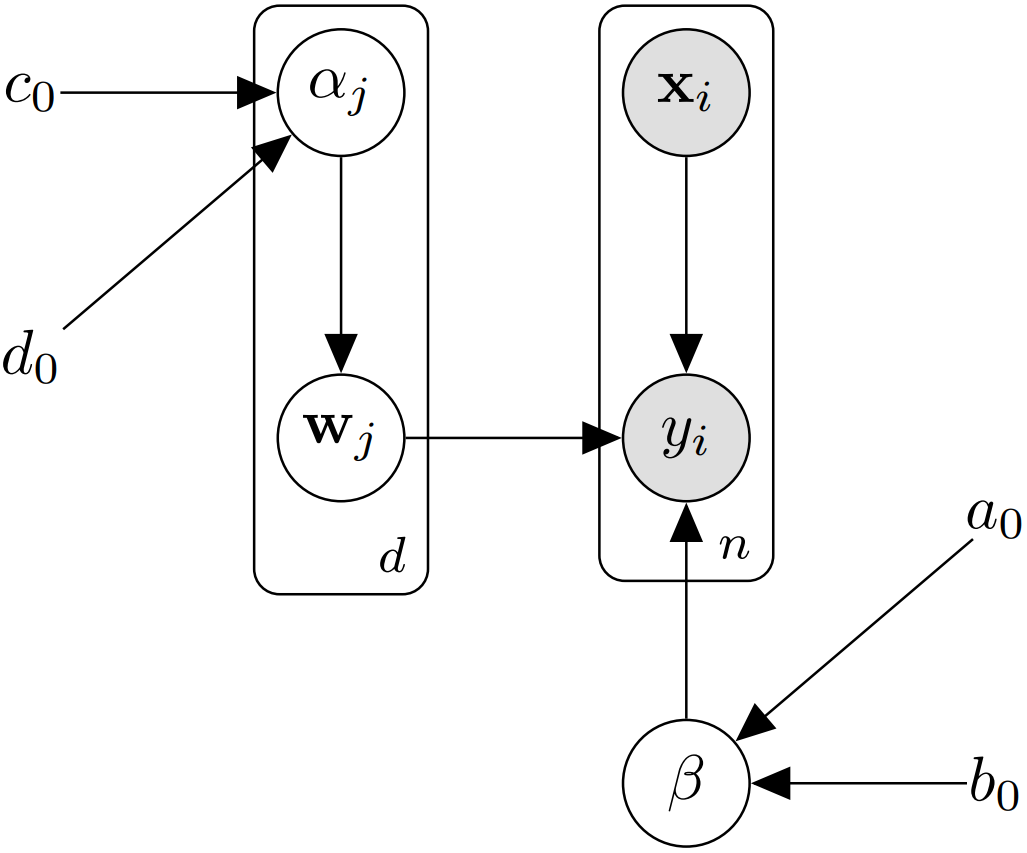
\includegraphics[width=0.5\textwidth]{bn_network.png}
        \caption{Plate diagram of the regression model with ARD prior. Variables $x_i$ , and $y_i$ are observed; We are interested in the posterior distribution of parameters $w$, $\alpha$ and $\beta$. The constants $a_0$ , $b_0$, $c_0$ , and $d_0$ are user-defined hyperparameters}
        \label{fig:diagram}
    \end{figure}

    The components so far can be represented as a Bayesian network, illustrated in Figure \ref{fig:diagram}. The posterior can be conveniently deducted from the diagram to be
    \begin{align*}
        P(w,\alpha,\beta|y,x) \propto \prodlim{1}{n}P(y_i|w,x_i,\beta)\prodlim[j]{1}{d}\enclb{P(w_j|\alpha_j)P(\alpha_j)}P(\beta). \numberthis\label{eq:posterior}
    \end{align*}

\section{Gibbs sampling and conjugate priors}
    Gibbs sampling will be used to approximate the optimal ARD regression model parameters. Gibbs sampler requires the full conditional distributions for the model parameters; $P(w|y,x,\alpha,\beta)$, $P(\alpha|y,x,w,\beta)$, $P(\beta|y,x,w,\alpha)$, where $\alpha=(\alpha_1,\ldots,\alpha_d)$.

    \subsection{Deriving conjugate prior for \texorpdfstring{$w$}{}}
        \begin{align*}
            %
            & P(w|y,x,\alpha,\beta) \propto \prodlim{1}{n}P(y_i|w,x_i,\beta) \prodlim[j]{1}{d}P(w_j|\alpha_j) \\
            & = N(y_i|X^Tw) \prodlim[j]{1}{d} N(w_j|0,(\sqrt{\alpha_j})^{-1})\\
            & \propto \exp\enclp{-\frac{1}{2}\beta(y-X^Tw)^T(y-X^Tw)} \prodlim[j]{1}{d} \exp\enclp{-\frac{1}{2} w^2(\sqrt{\alpha_j})^2} \\
            & = \exp\enclp{-\frac{1}{2}\beta(y-X^Tw)^T(y-X^Tw) - \frac{1}{2} \sumlim[j]{1}{d} w^2 \alpha} \\
            & = \exp\enclp{-\frac{1}{2}\beta(y-X^Tw)^T(y-X^Tw) - \frac{1}{2} w^T D w}
        \end{align*}
        where $D$ is a $d \times d$ diagonal matrix with the values $\alpha_1, \alpha_2, \ldots, \alpha_d$

        Completing the square seems reasonable at this point, now the goal is to complete the square, that is get the exponent in the form $\frac{1}{2}w^TAw+k^Tw$. For convenience we will take the logarithm to remove the base exponential:
        \begin{align*}
                %
                \Rightarrow \log P(w|y,x,\alpha,\beta) &\propto -\frac{1}{2}\beta \enclp{y^Ty - y^TX^Tw - w^TXy + w^TXX^Tw} - \frac{1}{2} w^T D w \\
                &\propto -\frac{1}{2} \enclb{-2\beta y^TX^Tw + \beta w^TXX^Tw} - \frac{1}{2} w^T D w \\
                &= \beta y^TX^Tw -\frac{1}{2} \beta w^TXX^Tw - \frac{1}{2} w^T D w \\
                &= -\frac{1}{2} \enclb{w^T\beta XX^Tw + w^T D w} + \beta y^TX^Tw \\
                &= -\frac{1}{2} w^T \undertext{\enclp{\beta XX^T + D}}{$=A$} w + \undertext{\beta y^TX^T}{$=k^T$}w
        \end{align*}

        Then by completing the square we obtain the parameters $S$ (covariance) and $m$ (mean) for a Multivariate Gaussian that is proportional to $P(w|y,x,\alpha,\beta)$:
        \begin{align*}
            S &= A^{-1} = \enclp{\beta XX^T + D}^{-1} \\
            m &= A^{-1}k = S \beta Xy\\
            &\dunderline{\Rightarrow P(w|y,x,\alpha,\beta) \propto \mathcal{N}(w|m,S)} \numberthis\label{eq:wconjugate}
        \end{align*}

    \subsection{Deriving conjugate prior for \texorpdfstring{$\alpha$}{}}
        \begin{align*}
            %
            P(\alpha|y,x,w,\beta) &\propto \prodlim[j]{1}{d}P(w_j|\alpha_j)P(\alpha_j) \\
            &= \prodlim[j]{1}{d} N(w_j|0,\alpha^{-1}) \opGamma(a_j|c_0,d_0) \\
            &\propto \prodlim[j]{1}{d} \frac{1}{\sqrt{\alpha_j^-1}} \exp\enclp{-\frac{1}{2} \enclb{\frac{w_j}{\sqrt{\alpha}^{-1}}}^2}\alpha_j^{c_0-1} \exp\enclp{-d_0\alpha_j} \\
            &= \prodlim[j]{1}{d} \exp\enclp{-\frac{w_j^2}{2}\alpha_j - d_0\alpha_j}\alpha_j^{c_0-1+1/2} \\
            &= \prodlim[j]{1}{d} \exp\enclp{-\alpha_j\enclp{\frac{w_j^2}{2}+d_0}}\alpha_j^{c_0-1+1/2} \\
            &\propto \dunderline{\prodlim[j]{1}{d} \opGamma(\alpha_j|c_0+\frac{1}{2},\frac{w_j^2}{2}+d_0)} \numberthis\label{eq:alphaconjugate}
        \end{align*}

        To sample an $\alpha_j$ from the distribution we simply sample from $\opGamma(\alpha_j|c_0-\frac{1}{2},\frac{w_j^2}{2}+d_0)$.

    \subsection{Deriving conjugate prior for \texorpdfstring{$\beta$}{}}
        \begin{align*}
            %
            P(\beta|y,x,w,\alpha) &\propto P(\beta)\prodlim{1}{n}P(y_i|w,x_i,\beta)\\
            &= \opGamma(\beta|a_0, b_0) \prodlim{1}{n}N(y_i|w^Tx_i,\sqrt{\beta^{-1}})\\
            &= \beta^{a_0-1} \exp\enclp{-b_0\beta} \prodlim{1}{n} \frac{1}{\sqrt{\beta^{-1}}} \exp\enclp{-\frac{1}{2}\enclp{\frac{y_i-w^Tx_i}{\sqrt{\beta^{-1}}}}^2} \\
            &= \beta^{a_0-1} \exp\enclp{-b_0\beta} \enclp{\beta^{1/2}}^n \exp\enclp{-\frac{1}{2}\sumlim{1}{n}\beta(y_i-w^Tx_i)^2} \\
            &= \beta^{a_0-1}\beta^{n/2}\exp\enclp{-b_0\beta-\frac{\beta}{2}\sumlim{1}{n}(y_i-w^Tx_i)^2} \\
            &= \beta^{a_0-1+n/2} \exp\enclp{-\beta\enclp{b_0+\frac{1}{2}\sumlim{1}{n}(y_i-w^Tx_i)^2}} \\
            & \dunderline{\propto \opGamma(\beta|a_0+n/2, b_0+\frac{1}{2}\sumlim{1}{n}(y_i-w^Tx_i)^2)} \numberthis\label{eq:betaconjugate}
        \end{align*}

    \subsection{Implementation}
        The core idea of the implementation is simple. To sample $w, \alpha, \beta$ we simply do:
        \begin{enumerate}
            \item Initialize $(w^{(1)}, \alpha^{(1)}, \beta^{(1)})$
            \item For $t=1,\ldots,T$
            \begin{enumerate}[label*={\arabic*.}]
                \item sample $w^{(t+1)} \sim P(w|\alpha^{(t)},\beta^{(t)})$
                \item sample $\alpha^{(t+1)} \sim P(\alpha|w^{(t+1)})$
                \item sample $\beta^{(t+1)} \sim P(\beta|w^{(t+1)})$
            \end{enumerate}
        \end{enumerate}


        The code is implemented in an object oriented style, and pseudocode below represents the source code. For simplicity of this task, the only basis functions available are polynomial kernels as Scikit-Learn has a class called PolynomialFeatures \cite{PolynomialFeatures} for them. The process of fitting a model to a given dataset $X$ and the labels $y$ primarily consists of two steps; the initialization phase, the sampling phase.

        Let $X$ be a dataset with $n$ number of data points with features $f_1, f_2, \ldots, f_d$.

        \subsubsection{Initialization phase}
            This phase consists of initializing the first values for the parameters. The initial values for $w, \alpha, \beta$ are sampled from
            \begin{algorithm}[H]
                \caption{LinearRegressionARD.init\_fit, method to initialize variables before fitting model using Gibbs sampling, Python-pseudocode}
                \label{alg:LinearRegressionARD}
                \begin{algorithmic}[1]
                    \REQUIRE {self, $X$: datapoints, $y$: labels, degree: polynomial degree, n\_gibbs: number of sampling iterations}
                    \STATE{self.X $\leftarrow$ preprocessed $X$ by using Scikit-Learn's PolynomialFeatures given polynomial degree}
                    \STATE{self.d $\leftarrow$ number of dimensions of the preprocessed $X$}
                    \algonewline{}
                    \STATE{self.ws $\leftarrow$ empty array with shape (n\_gibbs, self.d)}
                    \STATE{self.alphas $\leftarrow$ empty array with shape (n\_gibbs, self.d)}
                    \STATE{self.betas $\leftarrow$ empty array with shape (1, n\_gibbs)}
                    \algonewline{}
                    \STATE{// Initialize parameter values}
                    \STATE{self.ws[0] $\leftarrow$ sample self.d values from prior (\ref{eq:wprior})}
                    \STATE{self.alphas[0] $\leftarrow$ sample self.d values from prior (\ref{eq:betaprior})}
                    \STATE{self.betas[0] $\leftarrow$ sample a value from prior (\ref{eq:alphaprior})}
                \end{algorithmic}
            \end{algorithm}

        \subsubsection{Sampling phase}
            Directly following the initialization phase:
            \begin{algorithm}[H]
                \caption{LinearRegressionARD.fit, method to do Gibbs sampling, Python-pseudocode}
                \label{alg:LinearRegressionARD}
                \begin{algorithmic}[1]
                    \REQUIRE {self, $X$: datapoints, $y$: labels, n\_gibbs: number of sampling iterations}
                    \FOR {t=1 \TO t=n\_gibbs}
                        \STATE{self.ws[t] $\leftarrow$ sample self.d values from $P(w|\alpha^{(t-1)},\beta^{(t-1)})$}
                        \STATE{self.alphas[t] $\leftarrow$ sample self.d values from $P(\alpha|w^{(t)})$}
                        \STATE{self.betas[t] $\leftarrow$ sample a value from $P(\beta|w^{(t)})$}
                    \ENDFOR
                \end{algorithmic}
            \end{algorithm}

        \subsubsection{Parameters for finalized model} \label{seq:determine}
            Now, the goal is to do linear regression, i.e. we want a finalized model from our training that can be used for prediction. The sampling process will result with trace plots for the sampled parameters which we can visually inspect.
            \begin{figure}[H]
                \centering
                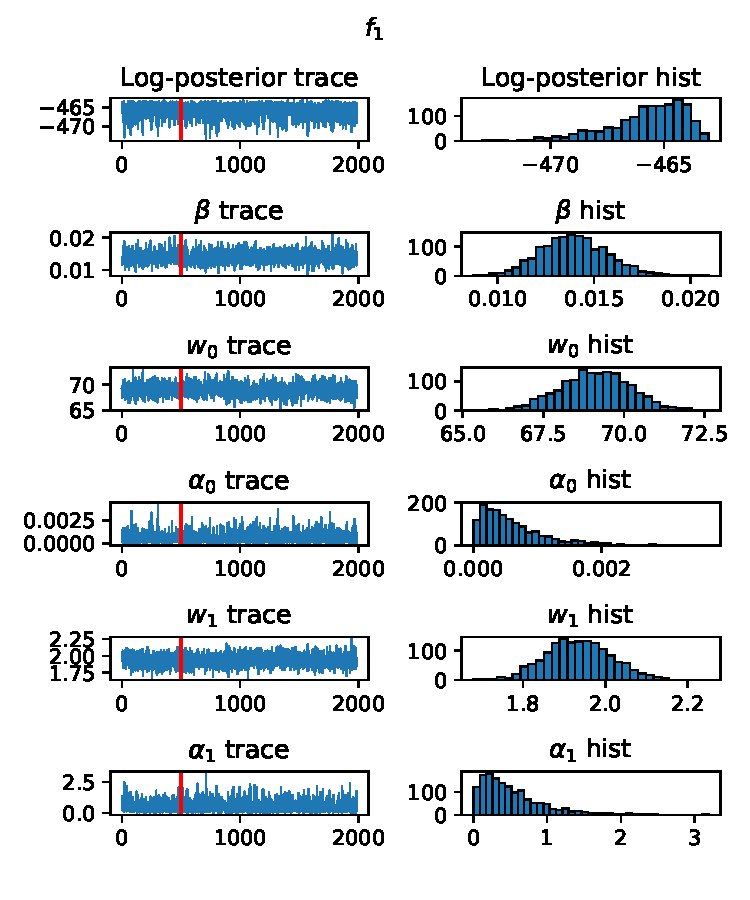
\includegraphics[width=0.48\textwidth]{f_1_noise0_tplot_ard.pdf}
                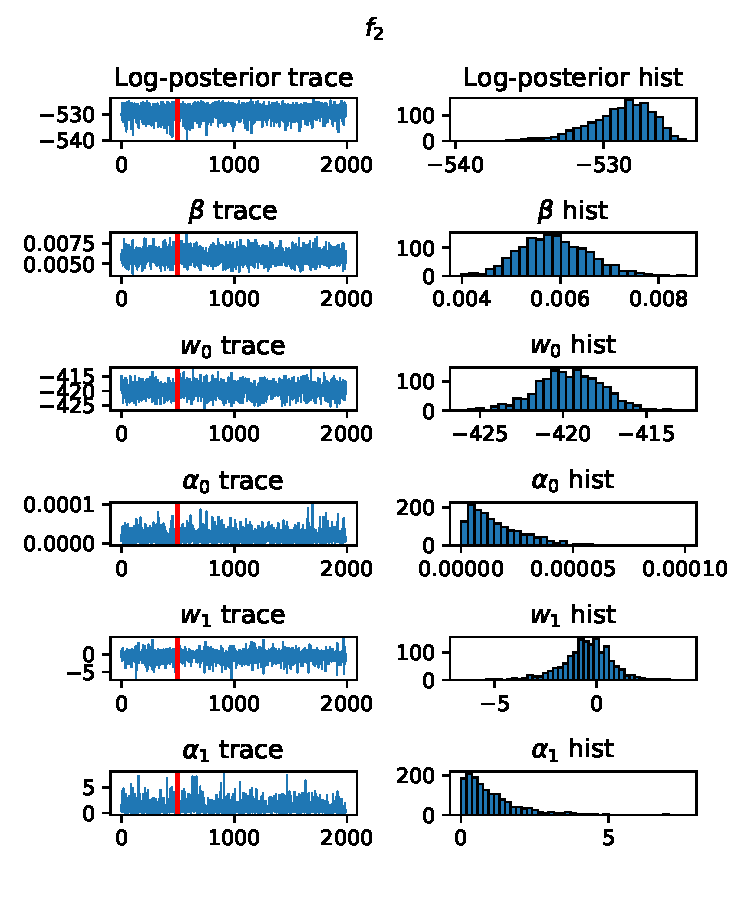
\includegraphics[width=0.48\textwidth]{f_2_noise0_tplot_ard.pdf}
                \caption{Here we see the trace plots using the implementation. Noisy data generated from the functions $f_1$ and $f_2$ are visualized in Figure \ref{fig:simfuncs} along with $f_1$ and $f_2$. The red line represents the fixed burnout cutoff of the first quarter of the samples. The histograms represents the distribution of samples after the cutoff. The sampling process in the plots consisted of 2000 iterations.}
            \end{figure}
            We are interested in the model weights $w_0, w_1, \ldots, w_d$. In order to determine what the final values for $w_0, w_1, \ldots, w_d$ should take we simply take the argmax of the histograms, i.e selecting the most frequent binned-value is sampled for each $w_i$. The motivation is that this is an discrete analogue to maximum likelihood. Hence we choose the most likely values, i.e. the most frequent ones. From visual inspection of the histograms, the argmax values are very reasonable and almost matches the true parameters for both $f_1$ and $f_2$ (see Figure \ref{fig:simfuncs}).

\section{Simulation study}
    To test the regression using ARD against the counterpart which does not use ARD we simulate some datasets to test on. The generated data will be generated using multivariate polynomials, as the implementations of the regression models are only capable of fitting polynomials.

    \subsection{The datasets}
        The simulated data will be generated from $8$ polynomial functions:
        \begin{align}
            f_1(x)&=2x+69 \label{eq:f1}\\
            f_2(x)&=4x^3+2x^2-420 \label{eq:f2}\\
            f_3(x,y)&=-4x+20y^2x+69 \label{eq:f3}\\
            f_4(x,y)&=69x+69y-420 \label{eq:f4}\\
            f_5(x,y)&=x^2-2y^2 \label{eq:f5}\\
            f_6(x,y)&=xy-x^2+y^2-420 \label{eq:f6}\\
            f_7(x,y)&=-x^3+42x^2-20x-y^3+42y^2-20y+69 \label{eq:f7}\\
            f_8(x,y)&=2x^3-y^3-3xy^2+3x^2y+x^3-3yx+69 \label{eq:f8}
        \end{align}

        The method of generating the data is simple. For each function $f_i$ do:
        \begin{enumerate}
            \item Randomly generate some data $X$ from the domain of $f_i$
            \item Obtain response values $y$ by inputting $X$ into $f_i$
            \item Offset each value of $y$ with gaussian noise (same noise distribution for all elements in $y$)
        \end{enumerate}

        The domain sampling distribution and noise distribution with respect for each function are as follows:
        \begin{table}[H]
            \centering
            \caption{Note that the domain distributions are univariate even though the some of the functions are multivariate. Values from the domain distributions are simply sampled repeatedly for each function variable, in this case $x$ and $y$.}
            \begin{tabular}{crr}
                \toprule
                function & domain distribution & noise distribution \\
                \midrule
                $f_1(x)$ & $\operatorname{Exp}(\text{rate}=10)$    & $N(0,9)$  \\
                $f_2(x)$ & $N(\text{mean}=-1.69, \text{std}=1.2)$    & $N(0,12)$  \\
                $f_3(x,y)$ & $\operatorname{Exp}(\text{rate}=5)$    & $N(0,22)$  \\
                $f_4(x,y)$ & $N(\text{mean}=69, \text{std}=4)$      & $N(0,420)$ \\
                $f_5(x,y)$ & $\operatorname{Unif}(\min=-2,\max=20)$ & $N(0,69)$  \\
                $f_6(x,y)$ & $N(\text{mean}=0, \text{std}=8)$       & $N(0,22)$  \\
                $f_7(x,y)$ & $\operatorname{Unif}(\min=-2,\max=36)$    & $N(0,420)$ \\
                $f_8(x,y)$ & $\operatorname{Unif}(\min=-6,\max=6)$  & $N(0,69)$  \\
                \bottomrule
            \end{tabular}
        \end{table}

        Then generating $128$ data samples for each function produces the following plots:
        \begin{figure}[H]
            \centering
            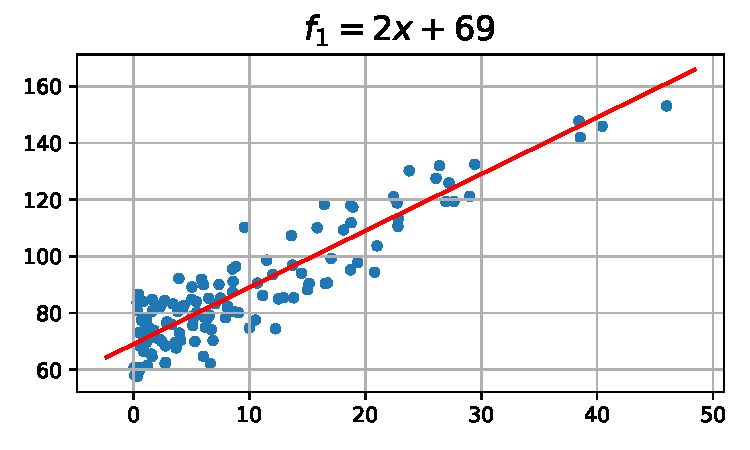
\includegraphics[width=0.45\textwidth, height=0.22\textheight]{f_1_2d.pdf}
            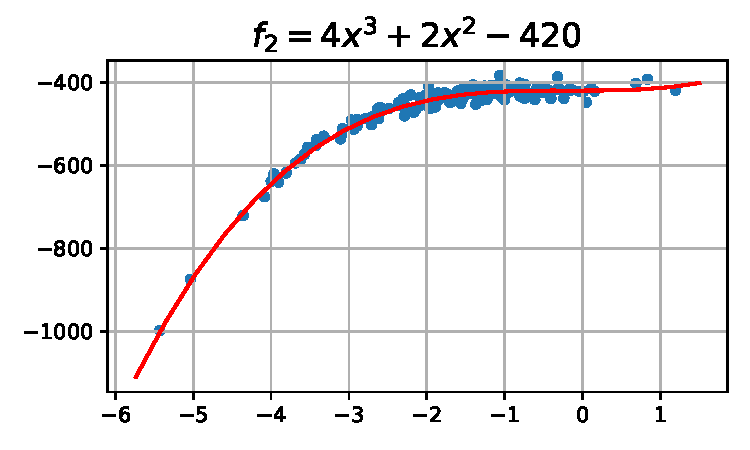
\includegraphics[width=0.45\textwidth, height=0.22\textheight]{f_2_2d.pdf}
            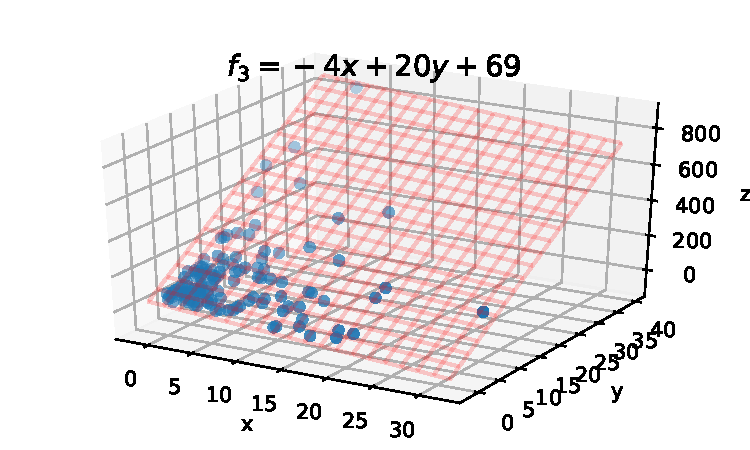
\includegraphics[width=0.45\textwidth, height=0.22\textheight]{f_3_3d.pdf}
            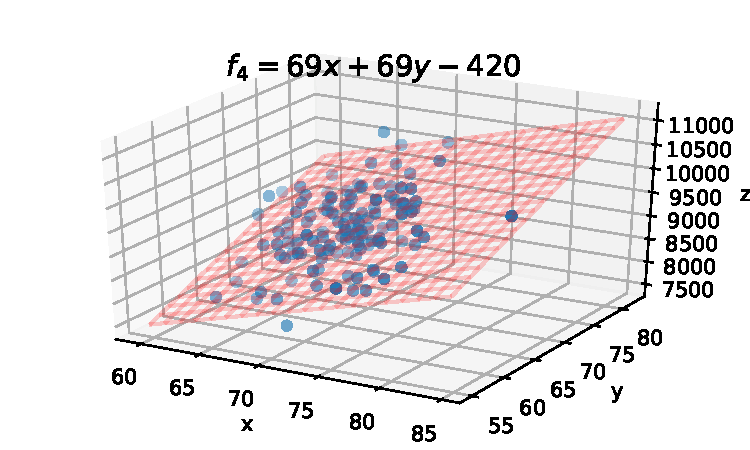
\includegraphics[width=0.45\textwidth, height=0.22\textheight]{f_4_3d.pdf}
            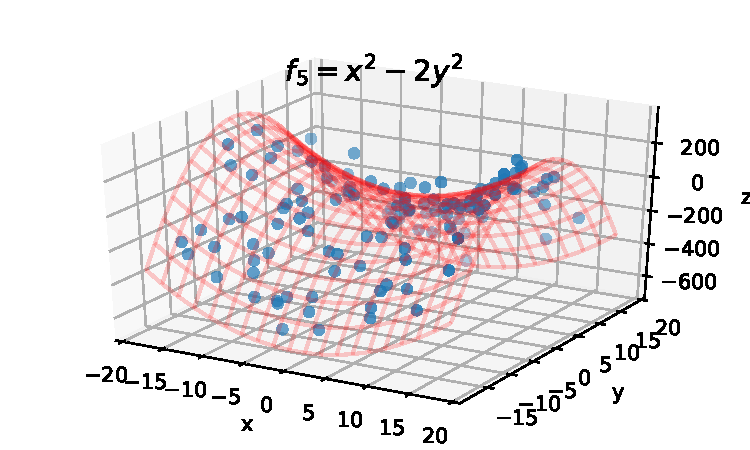
\includegraphics[width=0.45\textwidth, height=0.22\textheight]{f_5_3d.pdf}
            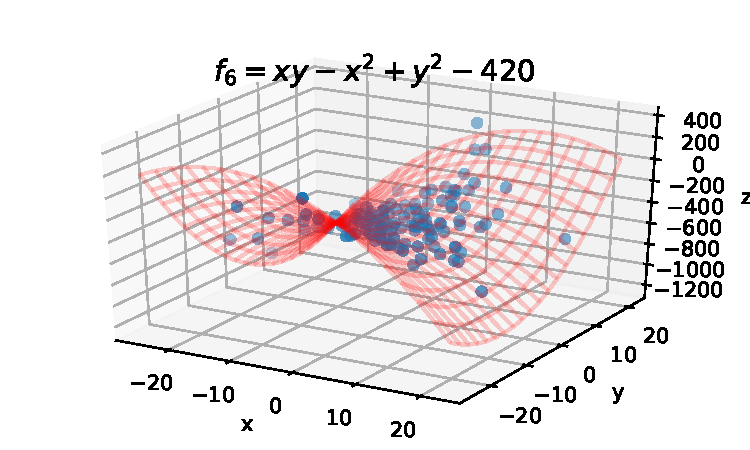
\includegraphics[width=0.45\textwidth, height=0.22\textheight]{f_6_3d.pdf}
            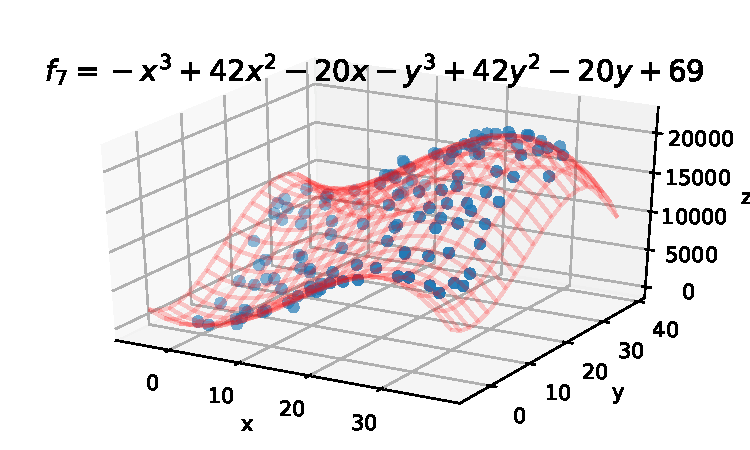
\includegraphics[width=0.45\textwidth, height=0.22\textheight]{f_7_3d.pdf}
            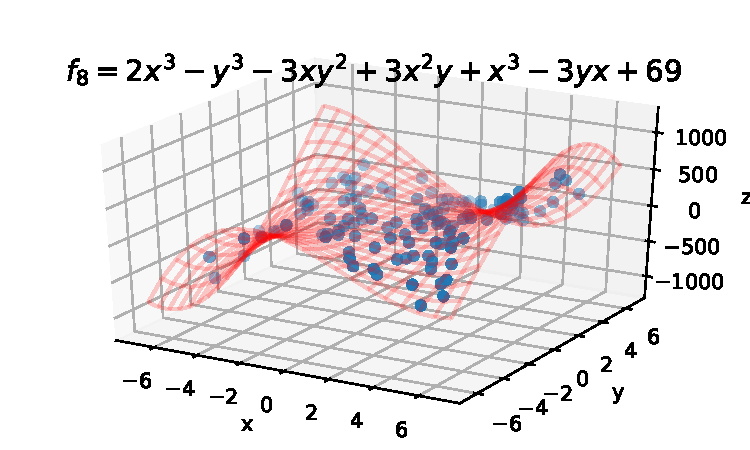
\includegraphics[width=0.45\textwidth, height=0.22\textheight]{f_8_3d.pdf}
            \caption{} \label{fig:simfuncs}
        \end{figure}

    \subsection{Regression on the generated data}
        We fit regression models using ARD and without ARD to assess the differences in performance. We use the mean absolute error on the data as performance metric. To assess the models' performances under presence of irrelevant features, we simply a add few extra features to the data that does not affect the response variables. The distribution of the noise features are sampled from:
        \begin{align*}
            N\enclp{\operatorname{Unif}\text{(min=-10, max=10)}, \operatorname{Unif}\text{(min=0.1, max=10)}}
        \end{align*}
        The number of sampling iterations is chosen to be $2000$ throughout this task. When training on the data, the models will be given the actual polynomial degree of the data. Any hyperparameters/user defined parameters are set to be 1 for the whole task for simplicity. The experiment should reveal how well the models manage to fit to training data given the actual polynomial degree. Formulated as a question; how well does the models manage to fit to data given the actual polynomial degree?

        \begin{table}[H]
            \centering
            \caption{"noise\_features" column indicates number of added irrelevant features to the data. The degree column indicates which degree the polynomial regression was done in. Bolded elements represents the one with the lowest MAE.}
            \begin{tabular}{llrrrr}
                \toprule
                  &       &  degree &  ARD\_MAE &  Regular\_MAE &  Regular\_over\_ARD \\
                noise\_features & function &         &          &              &                   \\
                \midrule
                0 & $f_1$ &       1 &     \textbf{7.05} &        43.55 &              6.17 \\
                & $f_2$ &       3 &    \textbf{10.62} &       403.08 &             37.96 \\
                & $f_3$ &       1 &    \textbf{18.08} &        99.23 &              5.49 \\
                & $f_4$ &       1 &   \textbf{342.17} &      8899.03 &             26.01 \\
                & $f_5$ &       2 &    55.64 &        \textbf{55.43} &              1.00 \\
                & $f_6$ &       2 &    \textbf{51.73} &       295.41 &              5.71 \\
                & $f_7$ &       3 &   \textbf{332.81} &      4631.12 &             13.92 \\
                & $f_8$ &       3 &    \textbf{58.82} &        71.39 &              1.21 \\
                \midrule
                1 & $f_1$ &       1 &   \textbf{7.06} &        40.56 &              5.75 \\
                & $f_2$ &       3 &    \textbf{10.32} &       266.15 &             25.78 \\
                & $f_3$ &       1 &    \textbf{18.15} &        96.93 &              5.34 \\
                & $f_4$ &       1 &   \textbf{347.15} &      8910.28 &             25.67 \\
                & $f_5$ &       2 &    \textbf{55.97} &        56.47 &              1.01 \\
                & $f_6$ &       2 &    \textbf{50.48} &       236.38 &              4.68 \\
                & $f_7$ &       3 &   \textbf{324.87} &      4499.19 &             13.85 \\
                & $f_8$ &       3 &    \textbf{56.19} &        71.78 &              1.28 \\
                \midrule
                2 & $f_1$ &       1 &   \textbf{7.99} &         8.41 &              1.05 \\
                & $f_2$ &       3 &    \textbf{11.51} &       274.97 &             23.90 \\
                & $f_3$ &       1 &    \textbf{18.22} &        77.85 &              4.27 \\
                & $f_4$ &       1 &   \textbf{355.07} &      8919.88 &             25.12 \\
                & $f_5$ &       2 &    63.10 &        \textbf{62.49} &              0.99 \\
                & $f_6$ &       2 &    \textbf{49.37} &       219.12 &              4.44 \\
                & $f_7$ &       3 &   \textbf{395.03} &      3565.01 &              9.02 \\
                & $f_8$ &       3 &    \textbf{68.88} &        64.46 &              0.94 \\
                \midrule
                3 & $f_1$ &       1 &    \textbf{7.69} &         8.40 &              1.09 \\
                & $f_2$ &       3 &   \textbf{12.72} &       120.63 &              9.48 \\
                & $f_3$ &       1 &   \textbf{18.25} &        99.53 &              5.45 \\
                & $f_4$ &       1 &  \textbf{352.42} &      8914.88 &             25.30 \\
                & $f_5$ &       2 &   53.55 &        \textbf{53.17} &              0.99 \\
                & $f_6$ &       2 &   \textbf{81.40} &        99.97 &              1.23 \\
                & $f_7$ &       3 &  \textbf{679.88} &      4405.54 &              6.48 \\
                & $f_8$ &       3 &   75.26 &        \textbf{58.70} &              0.78 \\
                \bottomrule
            \end{tabular}
        \end{table}

        Plots corresponding to the regression with no noise features and three noise features can be found in the appendix (Figure \ref{fig:appendixestimates} and \ref{fig:appendixestimates2}). After playing around with the functions and inspecting the results from the table, it seems to be that that regression without ARD struggles to estimate the intercept term, thus ruining its scores. Regression with ARD generally performed worse under the presence of noise features, but for some reason the version without ARD managed to get better with more noise features. Although it should be noted that we did not try to put a large number of noise features here, and it could simply be due to randomness. Generally, regression using ARD seems to be the best bet in general as it generally manages to get several times lower MAE values than without ARD. \\
        
        Implementation with ARD seems to fit well to the data, but without ARD seems to struggle with intercept term. 

        \begin{figure}[H]
            \centering
            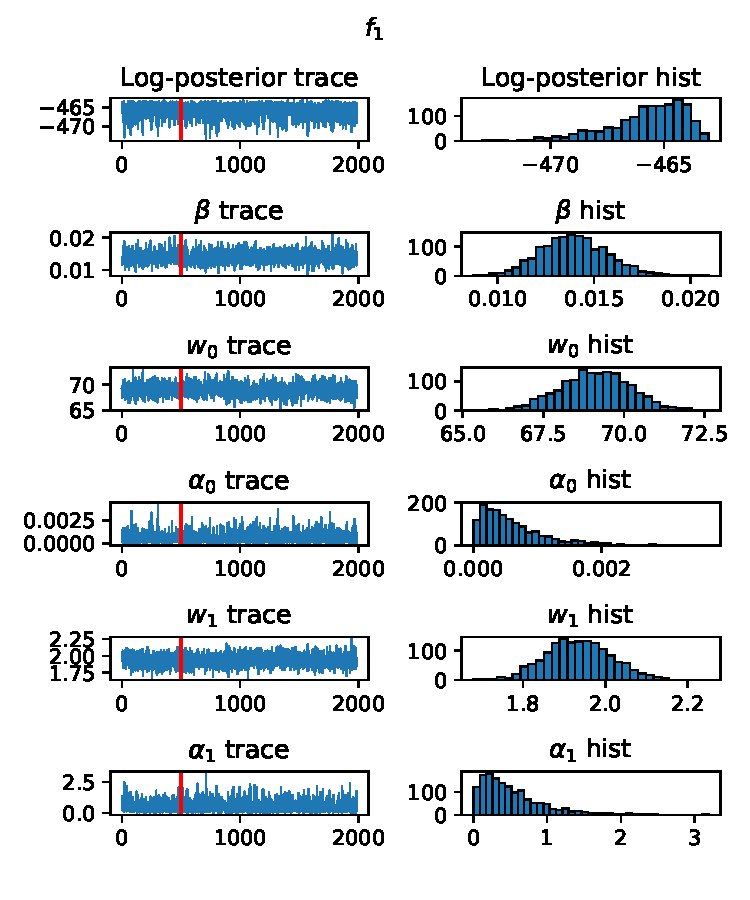
\includegraphics[width=0.45\textwidth]{f_1_noise0_tplot_ard.pdf}
            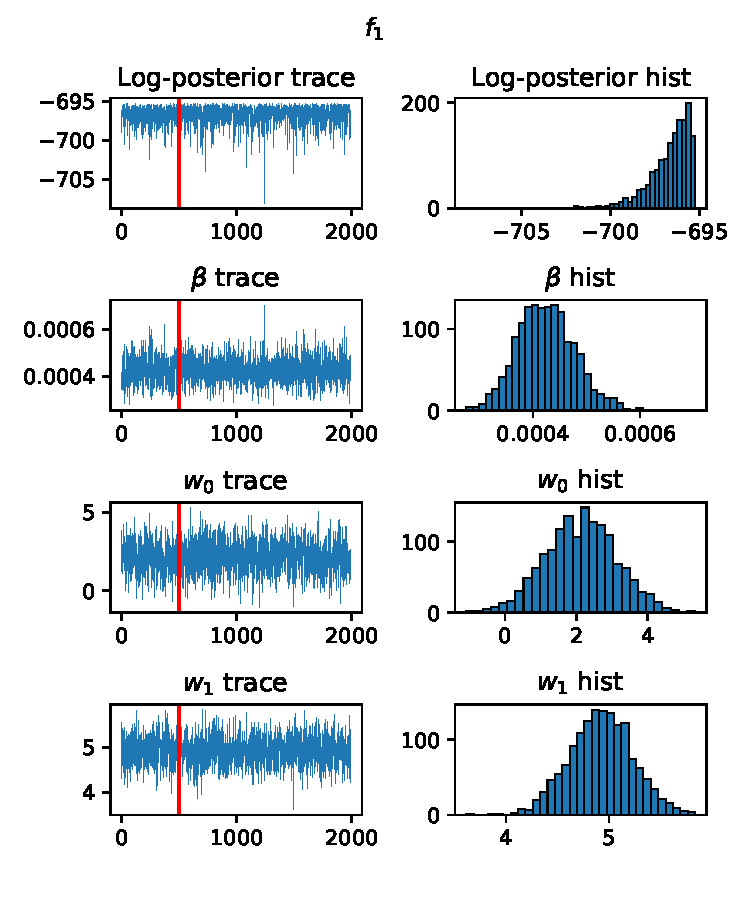
\includegraphics[width=0.45\textwidth]{f_1_noise0_tplot_reg.pdf}
            \caption{Left plot is ARD, right is without ARD. The true intercept for $f_1$ is $69$. We can see that the intercept ($w_0$) is mixing well for both, but the right plot (without ARD) does not converge to the correct value at all.}
        \end{figure}

    \section{Testing on real data}
    A real dataset is given to test the regression algorithms on. The dataset consists of 100 features. The selected polynomial degree to use is 1, as any higher degree will require infeasible computational times on my laptop. In order to assess which features are the most important we find the term with the highest polynomial absolute coefficient (ignoring the intercept term as it does not depend of any of the features). We assess this for both the model with and without ARD. 
    \begin{table}[H]
        \centering
        \caption{Feature importance in descending order of top five features.}
        \begin{tabular}{llr}
            \toprule
                        & Feature            &  coefficient \\
            \midrule
            with ARD & delta &        -2.60 \\
            & hsa.miR.29c. &         1.30 \\
            & hsa.miR.933 &        -1.19 \\
            & hsa.miR.328 &         1.09 \\
            & hsa.miR.24 &         0.88 \\
            \midrule
            without ARD & delta &        -2.60 \\
                        & hsa.miR.29c. &         1.30 \\
                        & hsa.miR.328 &         1.09 \\
                        & hsa.miR.770.5p &         0.44 \\
                        & hsa.miR.933 &        -1.19 \\
            \bottomrule
        \end{tabular}
    \end{table} 

    Both algorithms are agreeing on the two first features. Even the coefficient values are the same for the top two features. The features are delta and hsa.miR.29c. I would personally expect Age to play a bigger role, but it didn't apparently play that big of a role as we can see in the trace plots (Age coefficient is $w_2$).  Visualizing the first $15$ weights and variances shows that at least the first $15$ the parameters were mixing fine during the sampling process. As a reminder, the red vertical lines shows the cutoff value which is set to be at the first quarter of all the samples. Only the samples after the cut are used for determining the finalized values. It should be reasonable to assume that the rest of the parameters also mix well. 
    \begin{figure}[H]
        \centering
        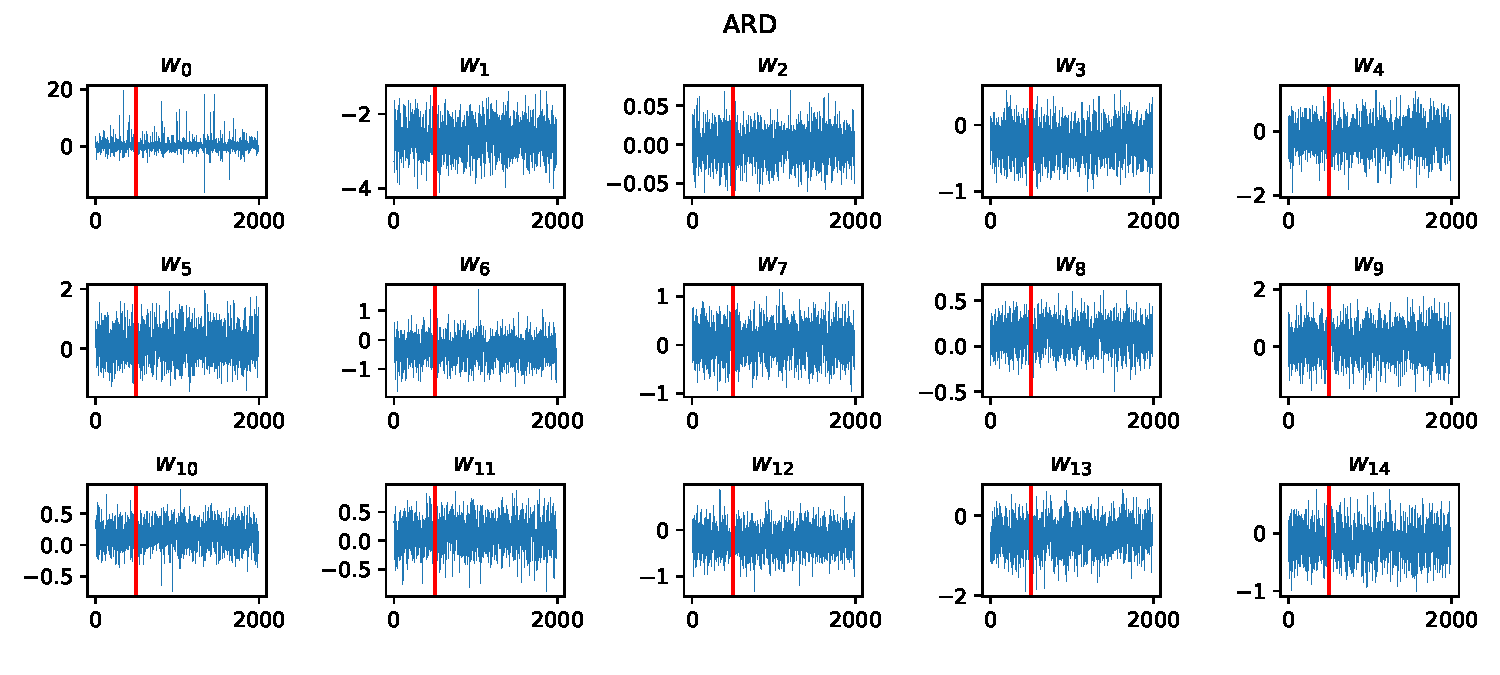
\includegraphics[width=0.9\textwidth]{real_w_traces_ard}
        \caption{Trace plots of first 15 regression weights from ARD model.}
    \end{figure}
    \begin{figure}[H]
        \centering
        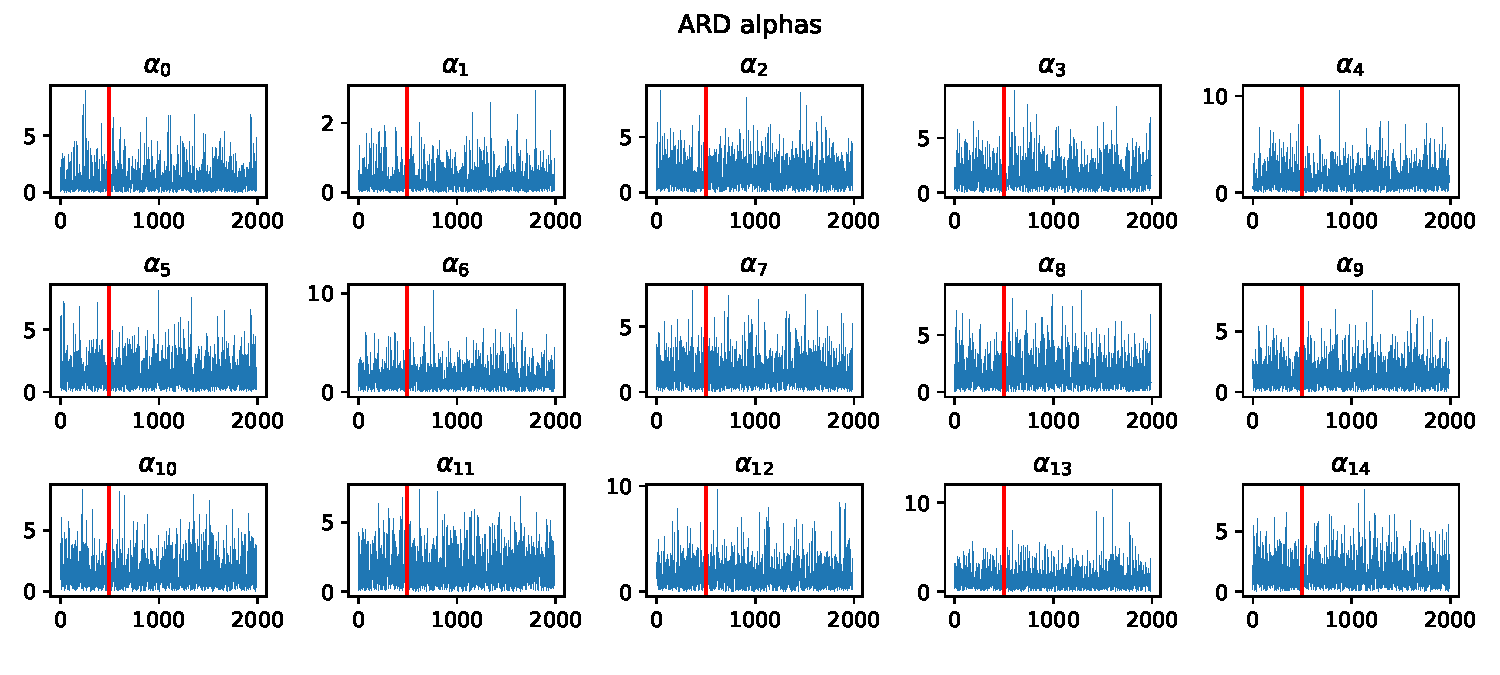
\includegraphics[width=0.9\textwidth]{real_alpha_traces_ard}
        \caption{Trace plots of first 15 alpha values from ARD model.}
    \end{figure}
    \begin{figure}[H]
        \centering
        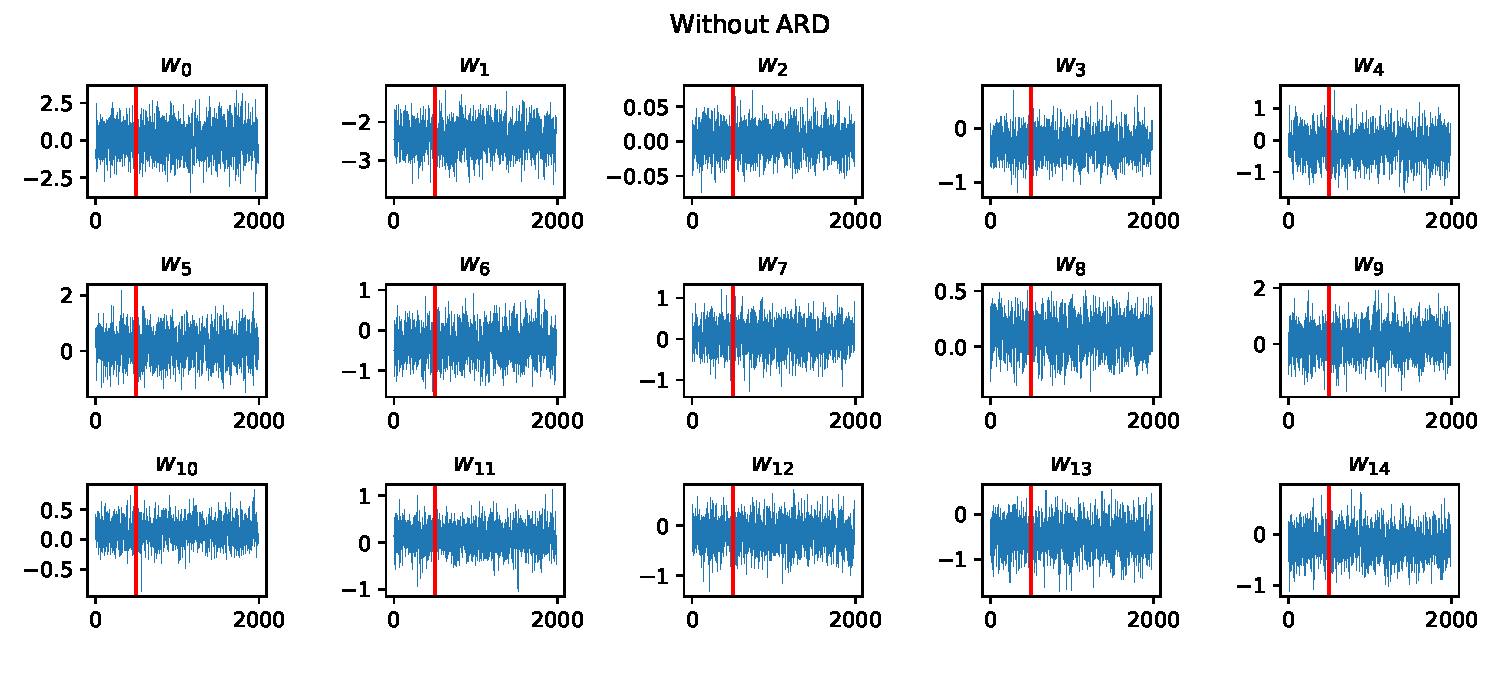
\includegraphics[width=0.9\textwidth]{real_w_traces_regular}
        \caption{Trace plots of first 15 regression weights from model without ARD.}
    \end{figure}

    The mean absolute errors for ARD and without were $33.71$ and $27.31$ respectively. The ARD model got beaten actually. Whether the difference is large or not dependents on the real noise distribution of the data.

    \section{Discussion}
        \subsection{Alternative to MAE on data as scoring metric}
        Using mean absolute error on the data as a scoring metric emphasizes the models' ability to fit to training data. An alternative metric would be to check how close the estimated model parameters were to the real parameters, i.e use MAE with respect to model parameters instead.

        \subsection{Approach to check for overfitting tendencies}
        The simulation part checked how the models manage to fit to the training data. Generally, polynomials model will tend to overfit if one assumes a polynomial degree higher than the actual function that the data was generated from. To check the tendency overfitting during such cases, we could try to fit high degree polynomial models with and without ARD, and then check the parameter loss between the estimated and actual polynomials.

        \subsection{Reason for struggling with intercept term}
        The implementation without ARD really struggled with estimating the intercept term. It should be noted that the intercept terms utilized in the simulation task were quite a bit larger than the other coefficients, and that is maybe why it struggled so much, but it still kind of odd that it would struggle this much. Further examination is needed.   

    \section{Conclusion}
    Fitting polynomial regression models using Gibbs sampling with ARD generally performs better than without ARD when specifying the actual polynomial degree of the polynomials the data was generated from. The method using Gibbs sampling to fit with polynomial kernels works fine for low dimensional data, but becomes very computationally heavy under the presence of many dimensions as the polynomial kernel increases in size polynomially. Linear regression without ARD seems to significantly struggle to estimate the intercept term. Both the algorithms works for the lung cancer data (when assuming polynomial of order one). The trace plots shows good mixing, and the it seems to be that the most important feature to predict the y-value is the delta feature.  

    \appendix
    \section{Estimates without noise features}
        \begin{figure}[H]
            \centering
            \caption{Left column is ARD, right column is without ARD} \label{fig:appendixestimates}
            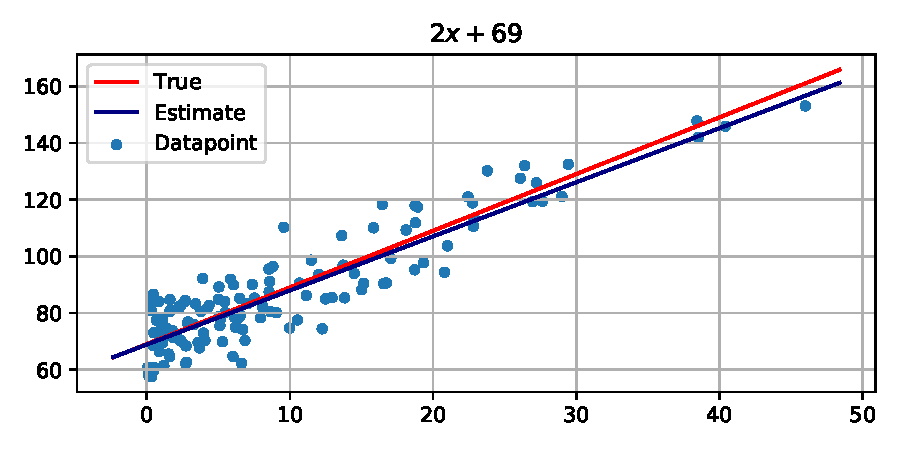
\includegraphics[width=0.45\textwidth]{f_1_noise0_estplot_ard}
            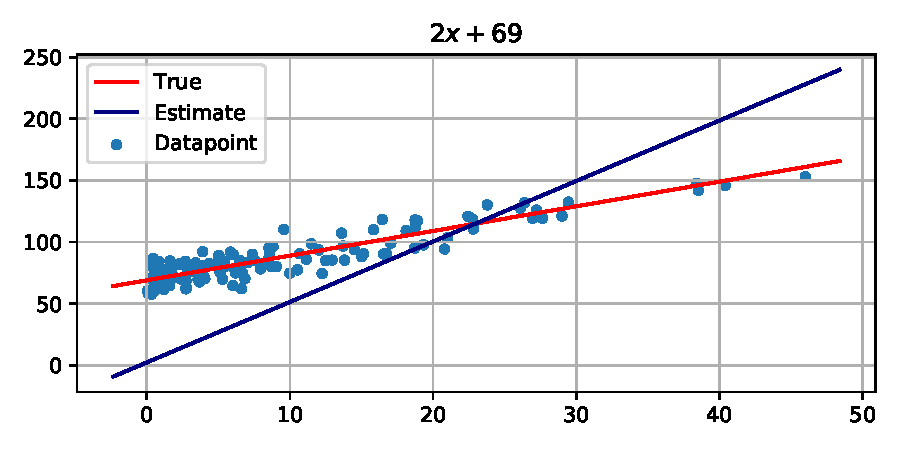
\includegraphics[width=0.45\textwidth]{f_1_noise0_estplot_regular}
            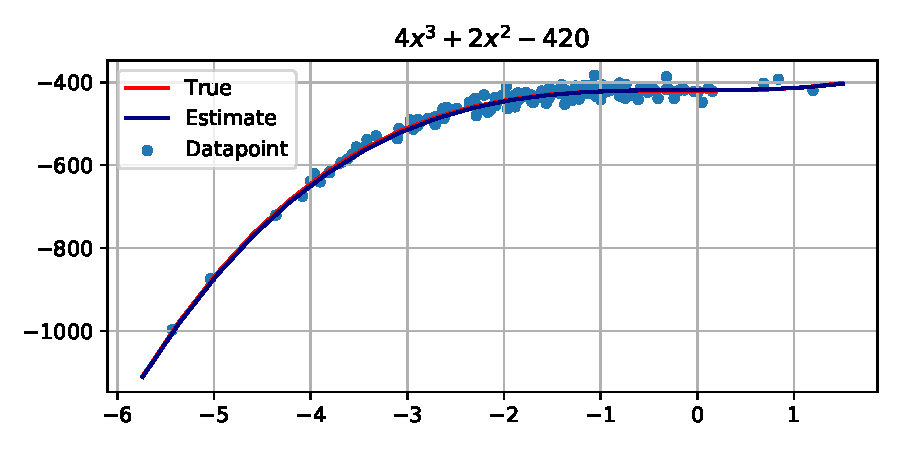
\includegraphics[width=0.45\textwidth]{f_2_noise0_estplot_ard}
            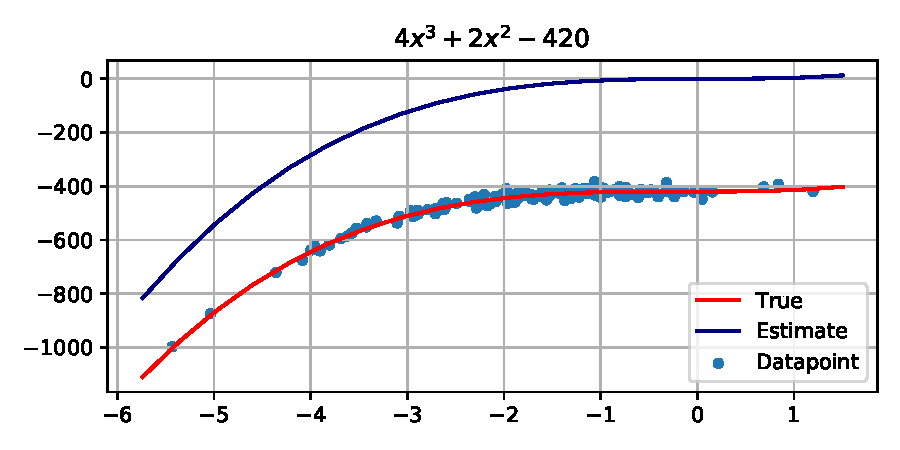
\includegraphics[width=0.45\textwidth]{f_2_noise0_estplot_regular}
            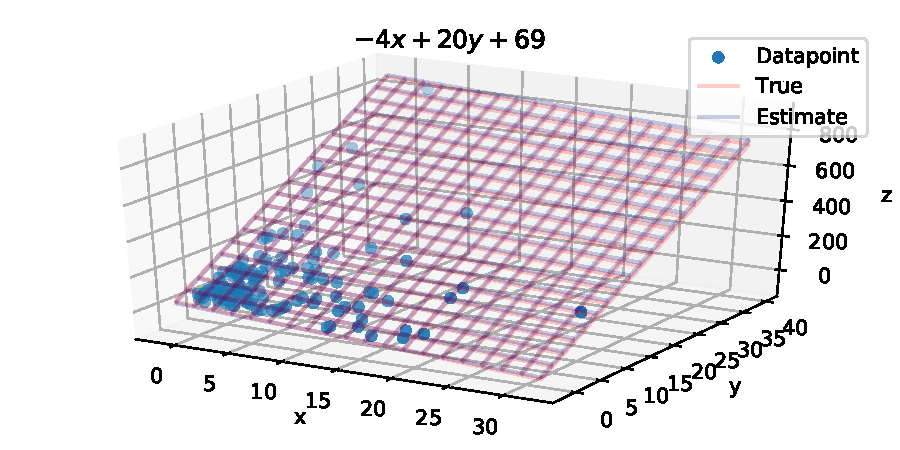
\includegraphics[width=0.45\textwidth]{f_3_noise0_estplot_ard}
            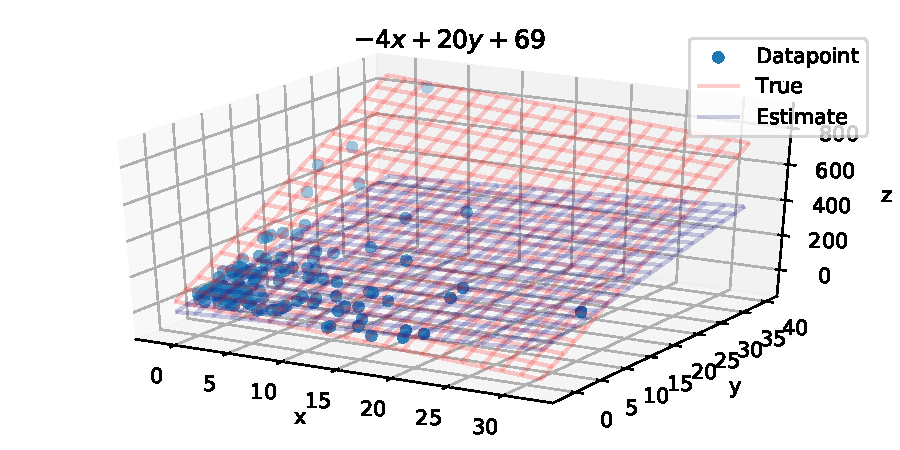
\includegraphics[width=0.45\textwidth]{f_3_noise0_estplot_regular}
            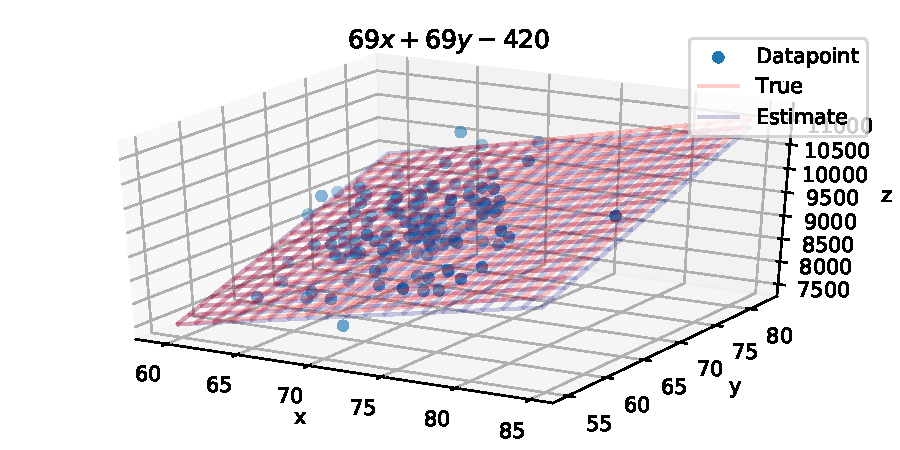
\includegraphics[width=0.45\textwidth]{f_4_noise0_estplot_ard}
            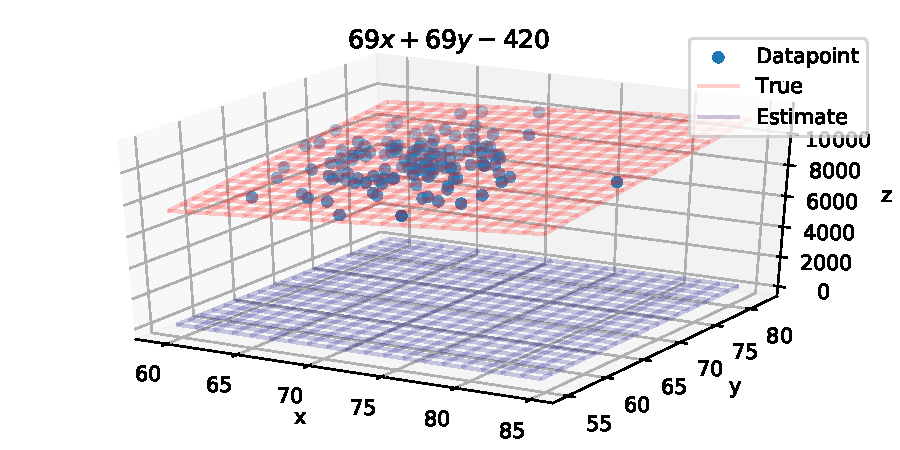
\includegraphics[width=0.45\textwidth]{f_4_noise0_estplot_regular}
        \end{figure}
        \begin{figure}[H]
            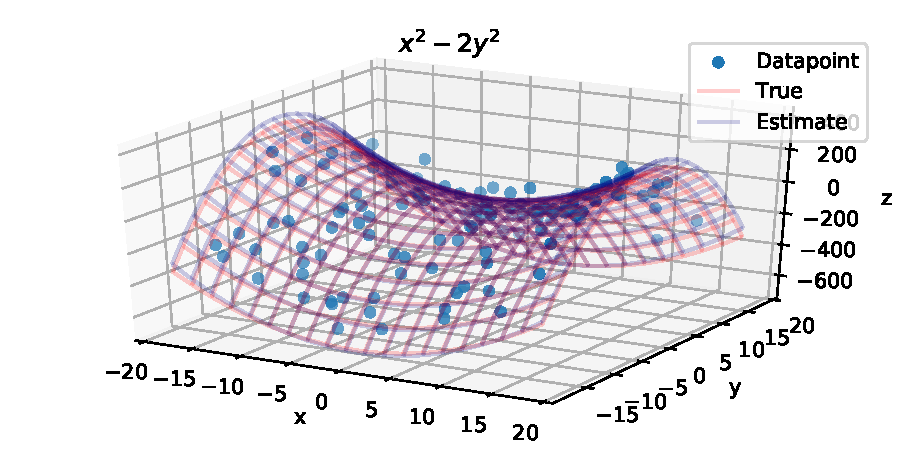
\includegraphics[width=0.45\textwidth]{f_5_noise0_estplot_ard}
            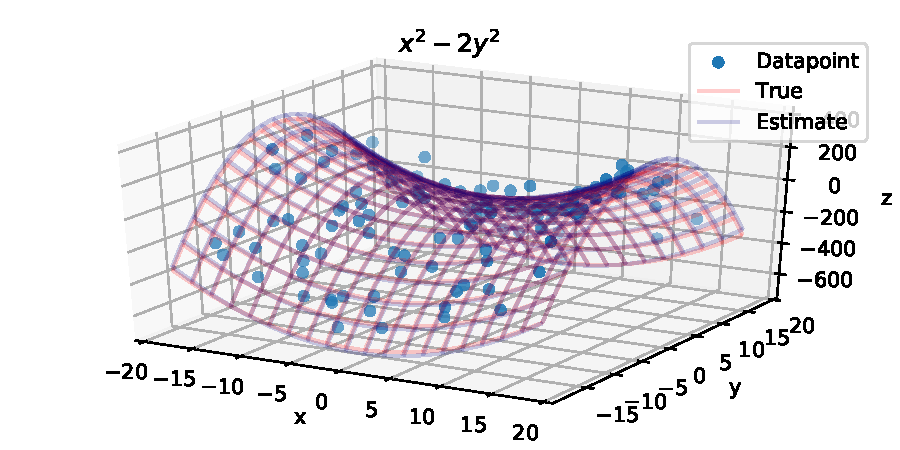
\includegraphics[width=0.45\textwidth]{f_5_noise0_estplot_regular}
            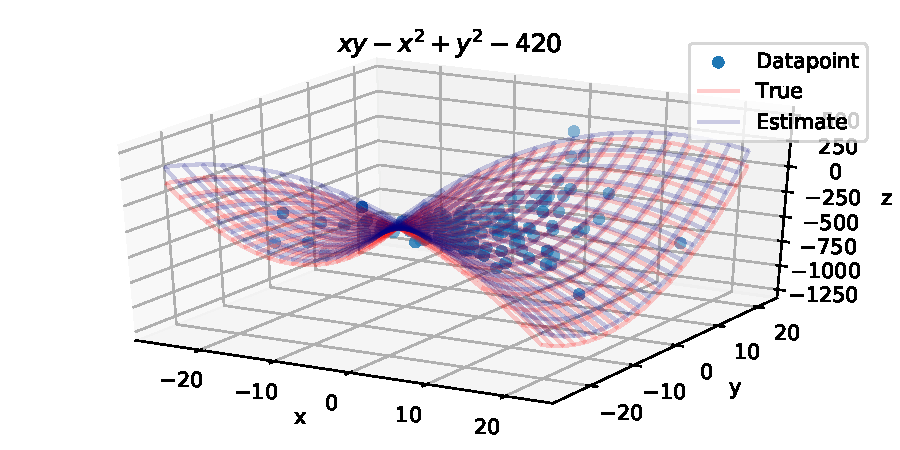
\includegraphics[width=0.45\textwidth]{f_6_noise0_estplot_ard}
            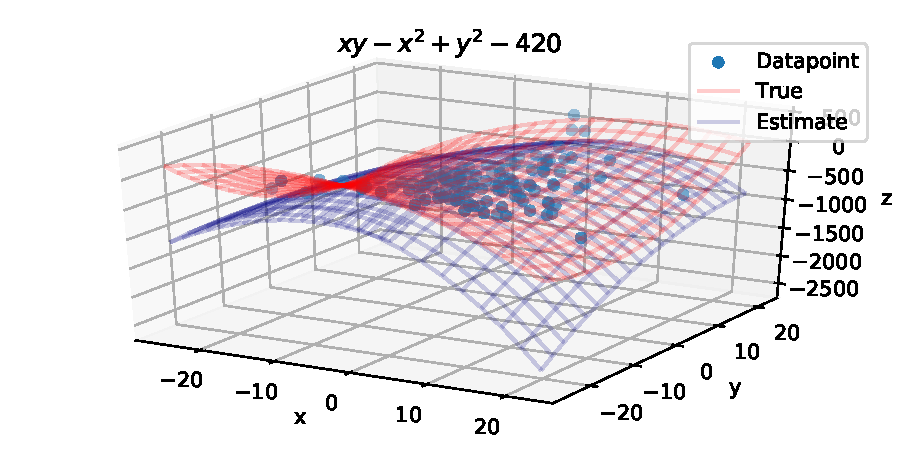
\includegraphics[width=0.45\textwidth]{f_6_noise0_estplot_regular}
            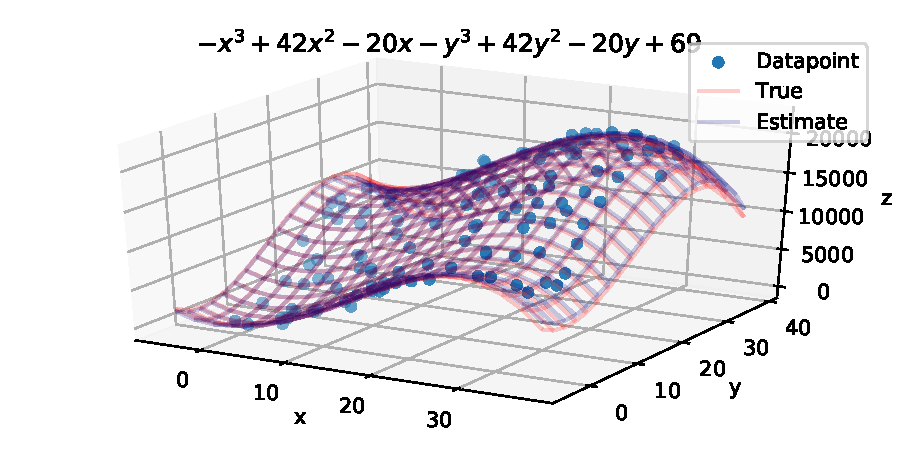
\includegraphics[width=0.45\textwidth]{f_7_noise0_estplot_ard}
            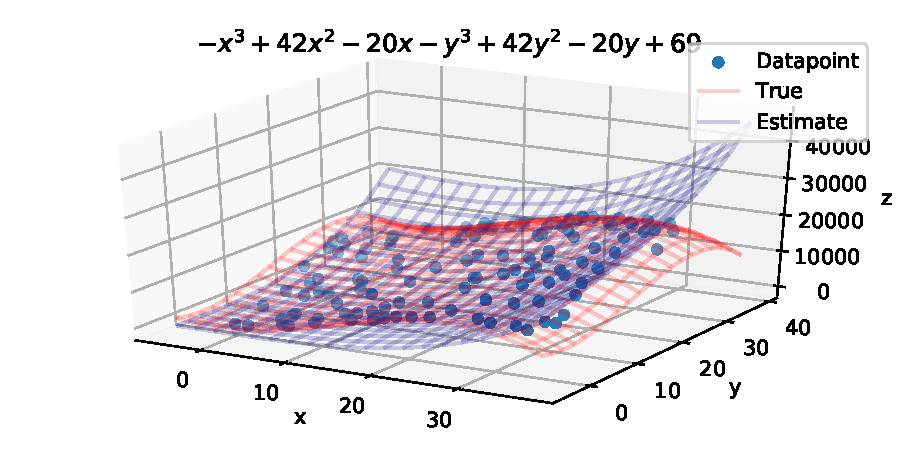
\includegraphics[width=0.45\textwidth]{f_7_noise0_estplot_regular}
            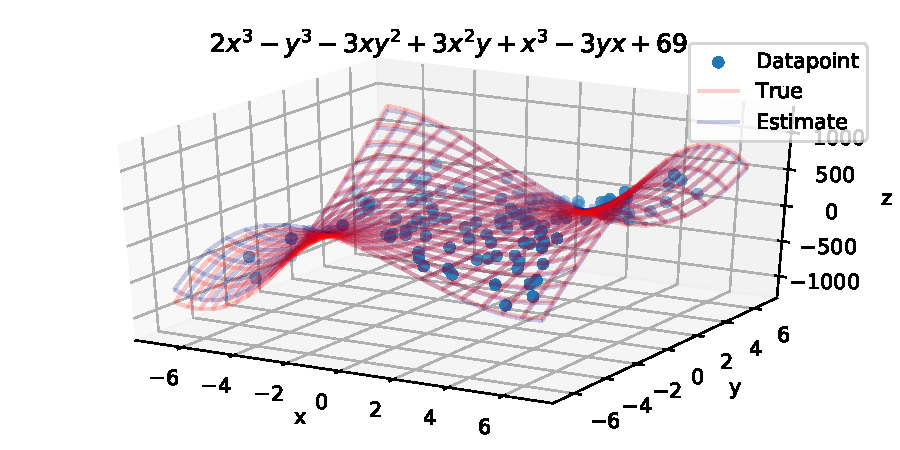
\includegraphics[width=0.45\textwidth]{f_8_noise0_estplot_ard}
            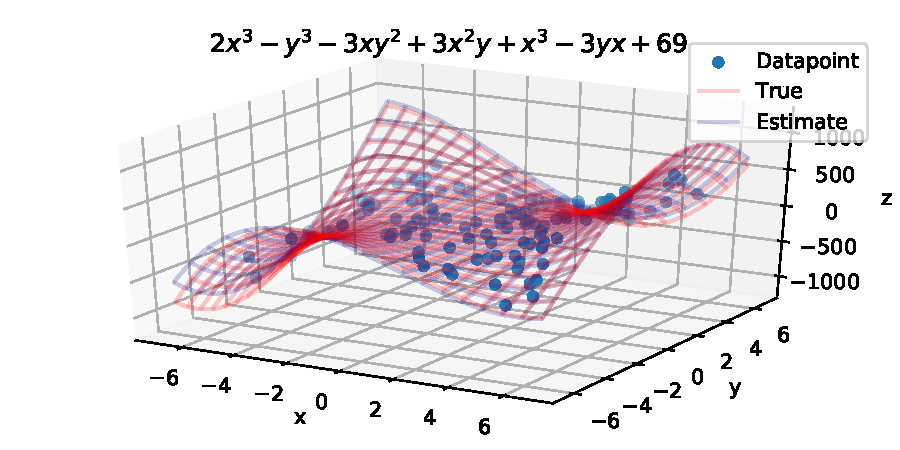
\includegraphics[width=0.45\textwidth]{f_8_noise0_estplot_regular}
        \end{figure}
    \section{Estimates with three noise features}
        \begin{figure}[H]
            \centering
            \caption{Left column is ARD, right column is without ARD} \label{fig:appendixestimates2}
            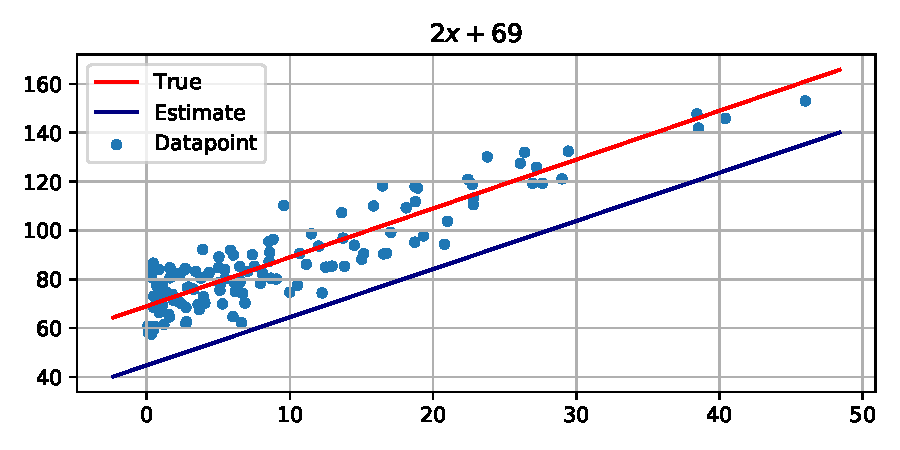
\includegraphics[width=0.45\textwidth]{f_1_noise3_estplot_ard}
            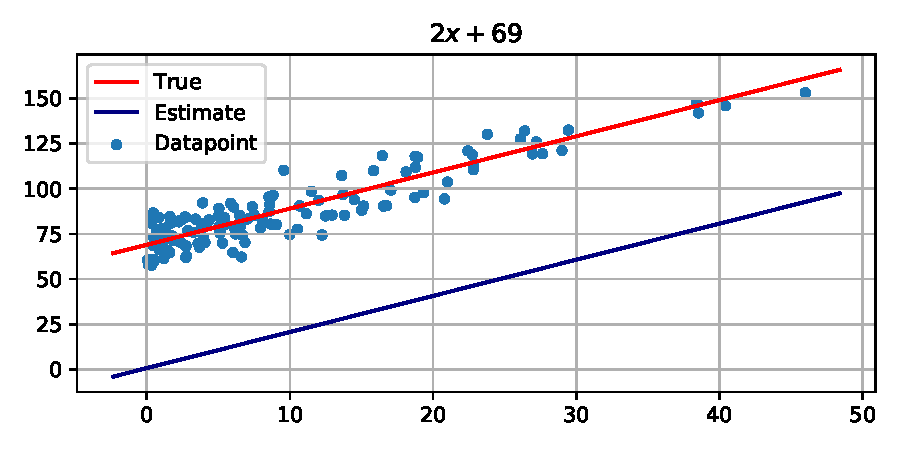
\includegraphics[width=0.45\textwidth]{f_1_noise3_estplot_regular}
            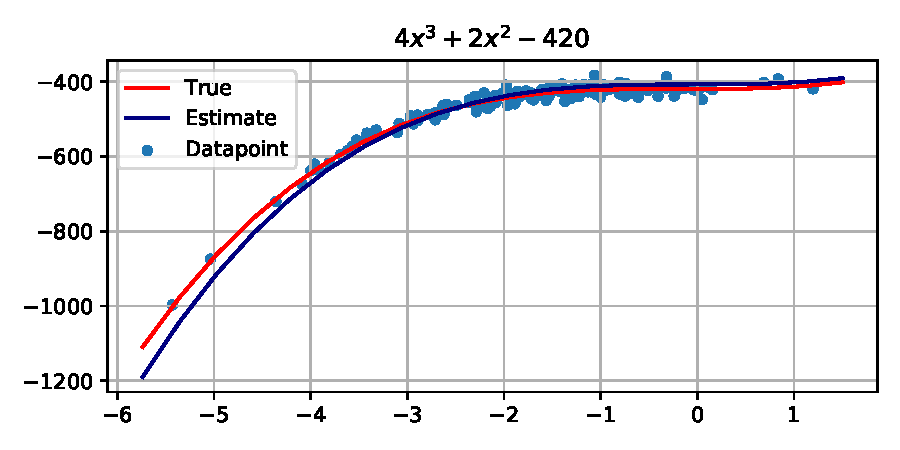
\includegraphics[width=0.45\textwidth]{f_2_noise3_estplot_ard}
            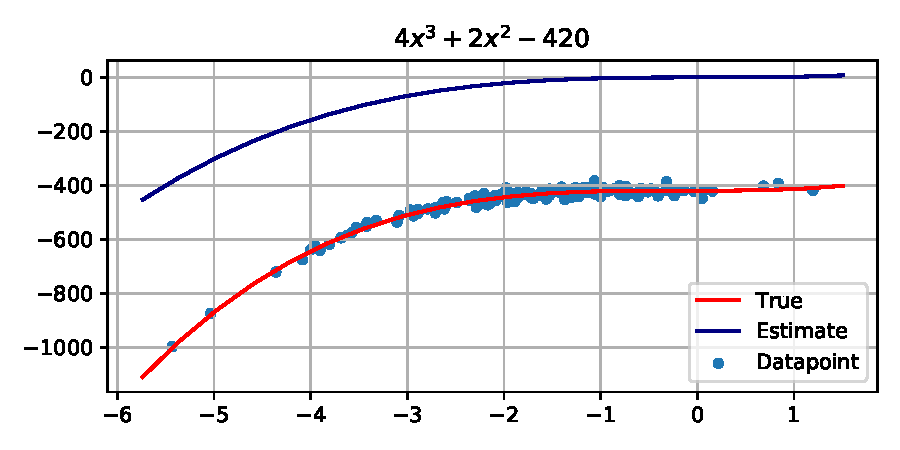
\includegraphics[width=0.45\textwidth]{f_2_noise3_estplot_regular}
            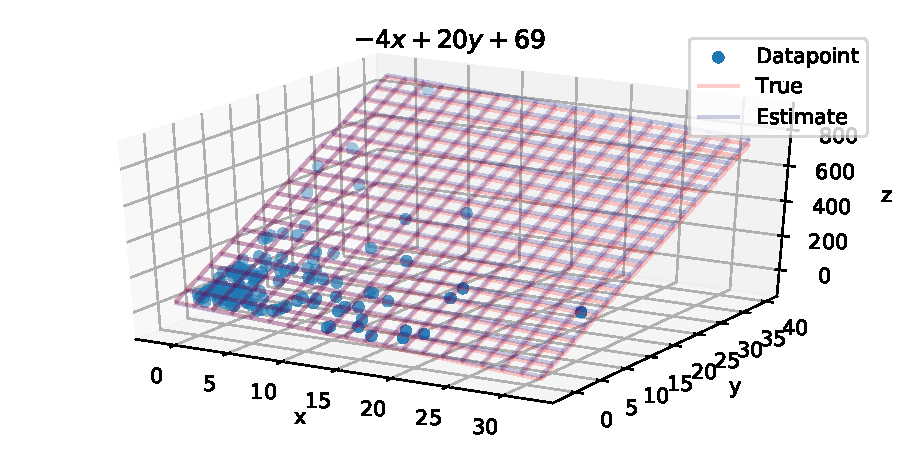
\includegraphics[width=0.45\textwidth]{f_3_noise3_estplot_ard}
            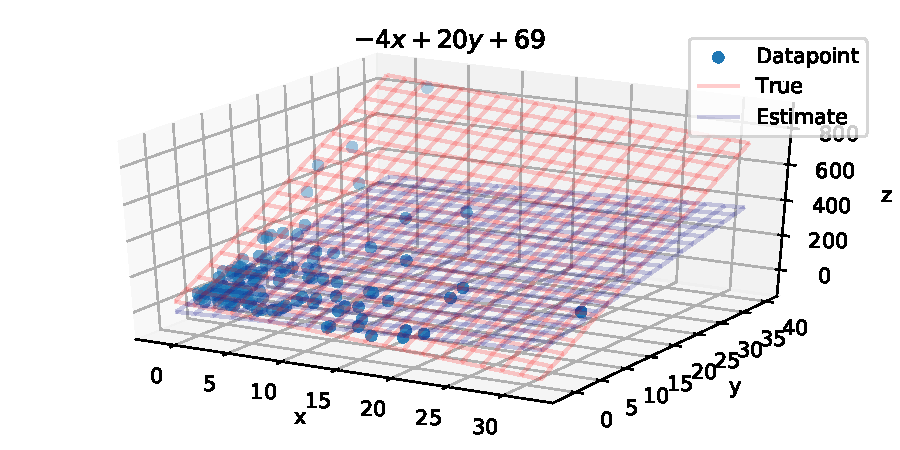
\includegraphics[width=0.45\textwidth]{f_3_noise3_estplot_regular}
            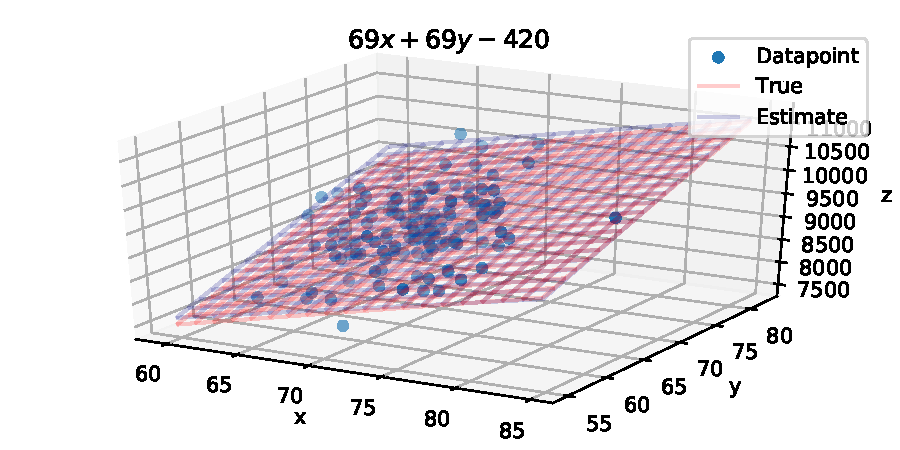
\includegraphics[width=0.45\textwidth]{f_4_noise3_estplot_ard}
            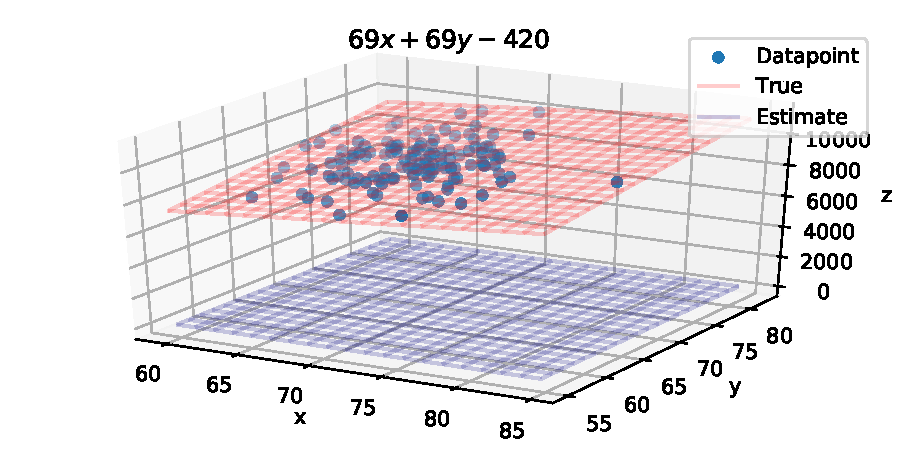
\includegraphics[width=0.45\textwidth]{f_4_noise3_estplot_regular}
        \end{figure}
        \begin{figure}[H]
            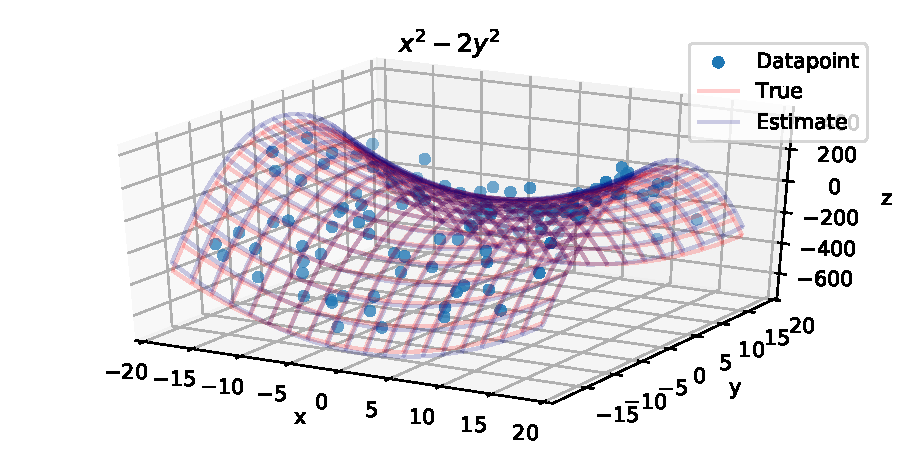
\includegraphics[width=0.45\textwidth]{f_5_noise3_estplot_ard}
            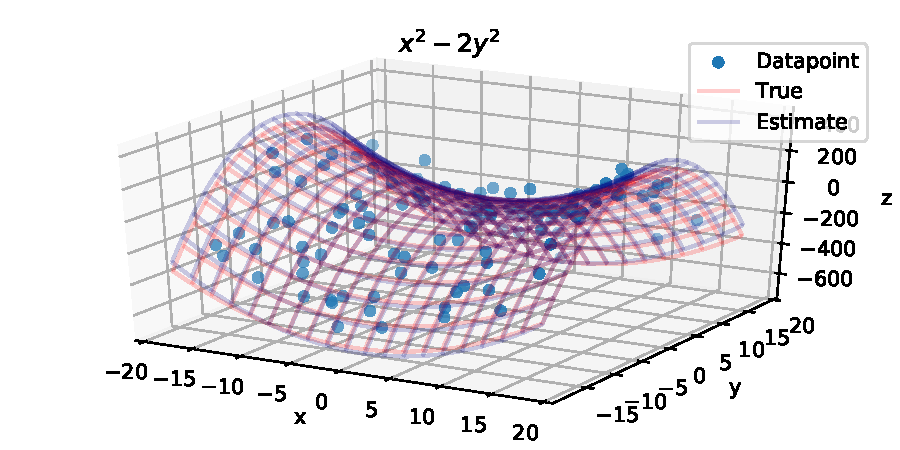
\includegraphics[width=0.45\textwidth]{f_5_noise3_estplot_regular}
            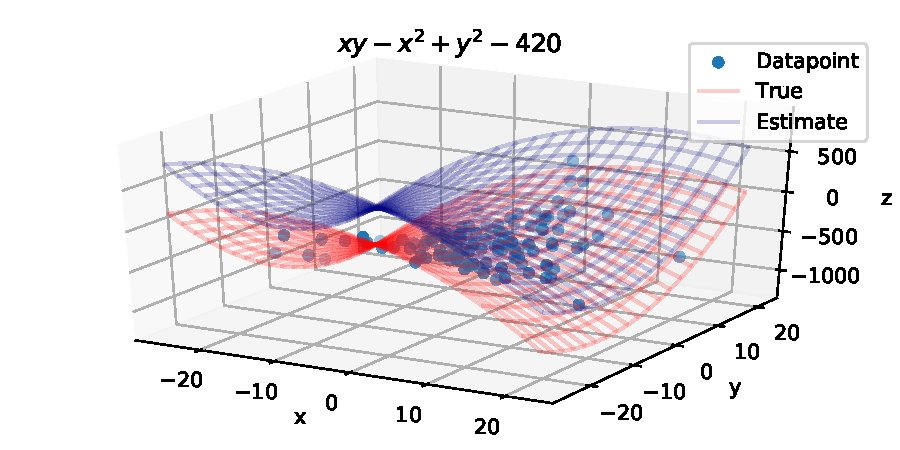
\includegraphics[width=0.45\textwidth]{f_6_noise3_estplot_ard}
            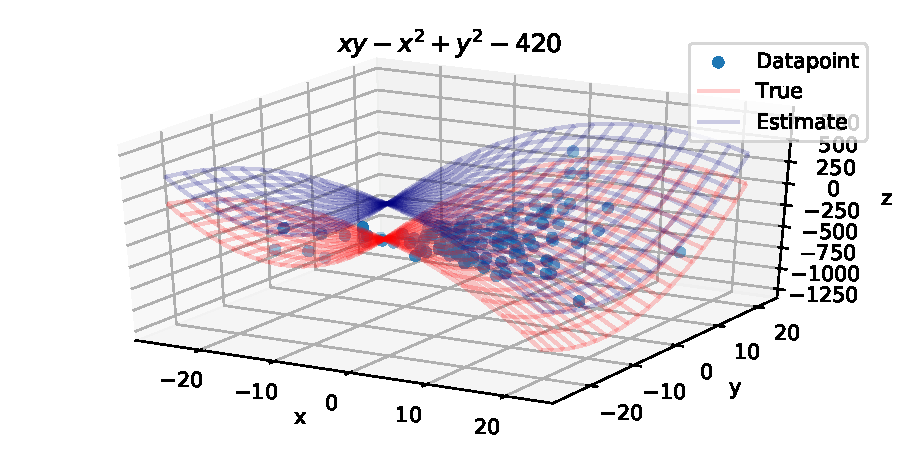
\includegraphics[width=0.45\textwidth]{f_6_noise3_estplot_regular}
            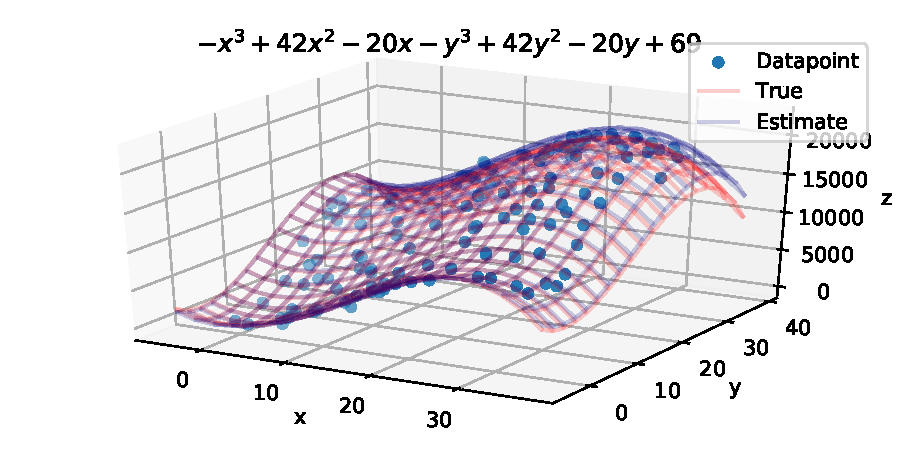
\includegraphics[width=0.45\textwidth]{f_7_noise3_estplot_ard}
            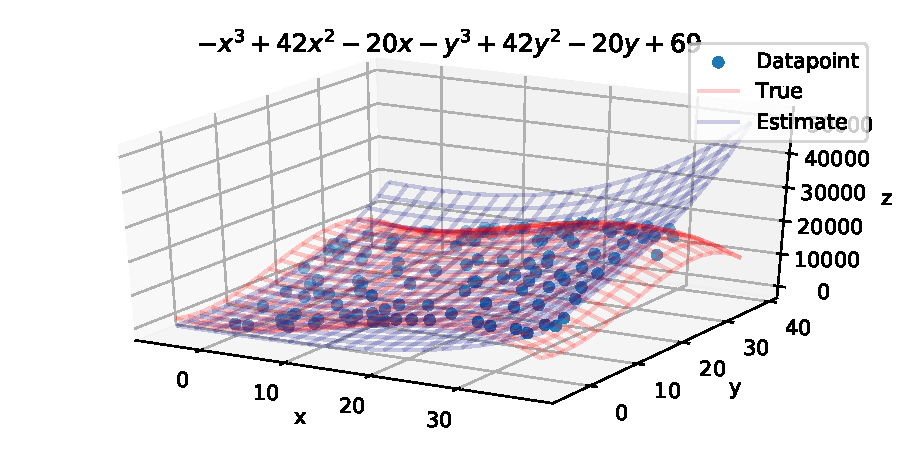
\includegraphics[width=0.45\textwidth]{f_7_noise3_estplot_regular}
            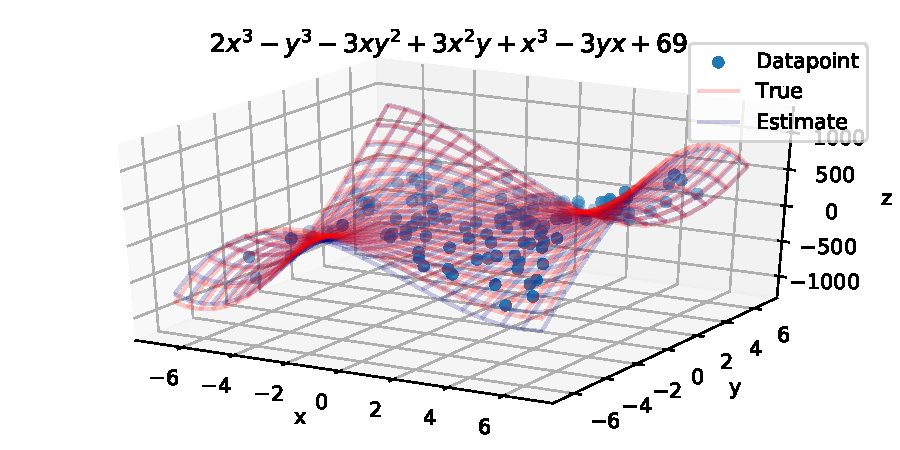
\includegraphics[width=0.45\textwidth]{f_8_noise3_estplot_ard}
            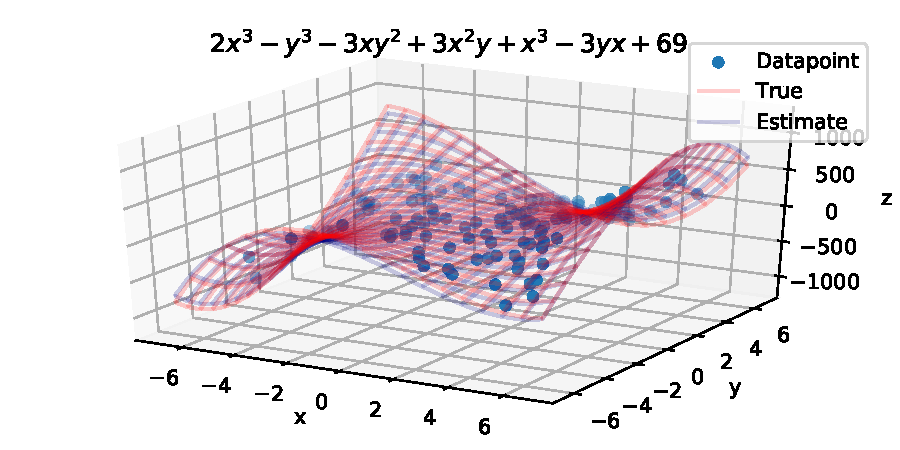
\includegraphics[width=0.45\textwidth]{f_8_noise3_estplot_regular}
        \end{figure}

    % \bibliographystyle{apalike}
    \bibliographystyle{ieeetran}
    \bibliography{citations}

    \end{document}
